
% \documentclass[journal]{template/vgtc}                     % final (journal style)
%\documentclass[journal,hideappendix]{template/vgtc}        % final (journal style) without appendices
\documentclass[review,journal]{template_ieee/vgtc}              % review (journal style)
%\documentclass[review,journal,hideappendix]{template/vgtc} % review (journal style)
%\documentclass[widereview]{template/vgtc}                  % wide-spaced review
%\documentclass[preprint,journal]{template/vgtc}            % preprint (journal style)

%% Uncomment one of the lines above depending on where your paper is
%% in the conference process. ``review'' and ``widereview'' are for review
%% submission, ``preprint'' is for pre-publication in an open access repository,
%% and the final version doesn't use a specific qualifier.

%% If you are submitting a paper to a conference for review with a double
%% blind reviewing process, please use one of the ``review'' options and replace the value ``0'' below with your
%% OnlineID. Otherwise, you may safely leave it at ``0''.
\onlineid{1820}

%% In preprint mode you may define your own headline. If not, the default IEEE copyright message will appear in preprint mode.
%\preprinttext{To appear in IEEE Transactions on Visualization and Computer Graphics.}

%% In preprint mode, this adds a link to the version of the paper on IEEEXplore
%% Uncomment this line when you produce a preprint version of the article 
%% after the article receives a DOI for the paper from IEEE
%\ieeedoi{xx.xxxx/TVCG.201x.xxxxxxx}

%% declare the category of your paper, only shown in review mode
\vgtccategory{Methodological paper}

%% please declare the paper type of your paper to help reviewers, only shown in review mode
%% choices:
%% * algorithm/technique
%% * application/design study
%% * evaluation
%% * system
%% * theory/model
\vgtcpapertype{application/design study}

%% Paper title.
% \title{Mind in Motion: EEG Correlates of Vection Induced During Acceleration in Virtual Reality}
\title{Towards the Automatic Detection of Vection in Virtual Reality Using EEG}
% \rs{Electrophysiological markers of accelleration and vection in Virtual Reality: Implicatins for cybersickeness}
%% Author ORCID IDs should be specified using \authororcid like below inside
%% of the \author command. ORCID IDs can be registered at https://orcid.org/.
%% Include only the 16-digit dashed ID.
%% This is how authors are specified in the conference style
\author{Gaël Van der Lee\thanks{e-mail: gael.vanderlee@univ-lille.fr}\\
    \scriptsize University of Lille
\and Anatole Lécuyer\\
    \scriptsize Inria Rennes\thanks{anatole.lecuyer@inria.fr}
\and Maxence Naud\\
    \scriptsize University of Lille
\and Reinhold Scherer\thanks{e-mail:r.scherer@essex.ac.uk}\\
     \scriptsize University of Essex
\and François Cabestaing\thanks{e-mail:francois.cabestaing@univ-lille.fr}\\
    \scriptsize University of Lille
\and Hakim Si-Mohammed\thanks{e-mail:hakim.simohammed@univ-lille.fr}\\
    \scriptsize University of Lille}


%% Abstract section.
\abstract{%
  Cybersickness remains a major barrier to the widespread adoption of virtual reality (VR).
Current subjective questionnaires are retrospective and insufficient for the dynamic, continuous assessment required to diagnose its determinants and implement real-time mitigation.

To address this, the field has increasingly investigated neuromarkers: signals derived from non-invasive neuroimaging as well as neurostimulation.
This PRISMA-guided systematic review synthesizes 92 studies investigating the neurophysiology of cybersickness in VR.
The corpus explicitly unites recording modalities (77 electroencephalography, 4 functional near-infrared spectroscopy) with neurostimulation interventions (11 studies spanning galvanic vestibular, transcranial direct-current, and transcranial alternating-current stimulation) under a unified frame.

Synthesis of the literature reveals consistent neural correlates alongside a critical methodological confound.
Cybersickness is predominantly associated with increased low-frequency (delta and theta) power and decreased alpha-band power.
However, we report meta-analytic evidence that VR hardware significantly modulates these band-power responses ($p=0.004$ on alpha, large effect; $p=0.015$ on beta), indicating that prior contradictions in the literature are partly attributable to hardware confounds rather than to differences in cybersickness per se.

Despite these advances, the literature faces substantial methodological and reporting barriers.
A methodological audit of the 38 classification or prediction studies reveals sparse reporting and arbitrary thresholds: only one study reports leave-one-subject-out validation, nineteen do not disclose a sick-versus-non-sick decision threshold, and thirteen report accuracy without sensitivity, specificity, AUC, or F1.
We conclude with a call for standardized reporting, multi-site open data, and causal validation via interventional designs to establish robust neuromarkers that can enable adaptive, user-aware immersive systems.

  %
  %% We recommend that you link to your supplemental material here in the abstract, as well
  %% as in the Supplemental Materials section at the end.
  
}

%% Keywords that describe your work. Will show as 'Index Terms' in journal
%% please capitalize first letter and insert punctuation after last keyword
\keywords{Human-centered computing, Human computer interaction (HCI), Interaction paradigms, Virtual reality}

%% A teaser figure can be included as follows
% \teaser{
%   \centering
%   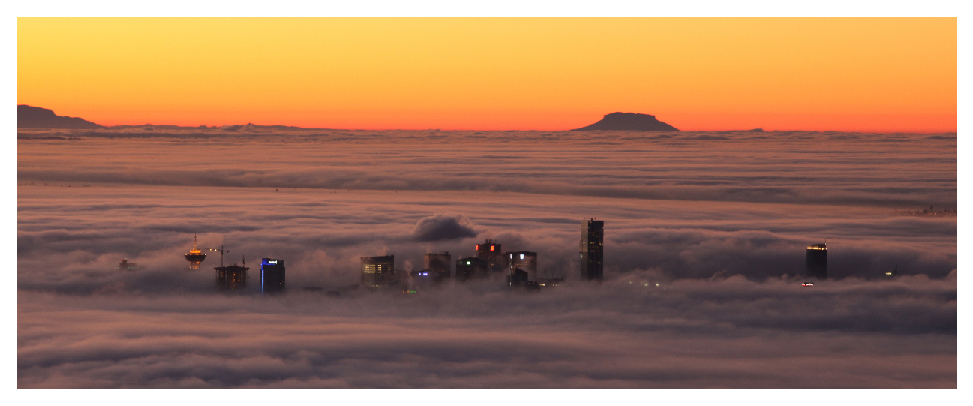
\includegraphics[width=\linewidth, alt={A view of a city with buildings peeking out of the clouds.}]{CypressView}
%   \caption{%
%   	In the Clouds: Vancouver from Cypress Mountain.
%   	Note that the teaser may not be wider than the abstract block.%
%   }
%   \label{fig:teaser}
% }

%% Uncomment below to disable the manuscript note
%\renewcommand{\manuscriptnotetxt}{}

%% Copyright space is enabled by default as required by guidelines.
%% It is disabled by the 'review' option or via the following command:
%\nocopyrightspace


%%%%%%%%%%%%%%%%%%%%%%%%%%%%%%%%%%%%%%%%%%%%%%%%%%%%%%%%%%%%%%%%
%%%%%%%%%%%%%%%%%%%%%% LOAD PACKAGES %%%%%%%%%%%%%%%%%%%%%%%%%%%
%%%%%%%%%%%%%%%%%%%%%%%%%%%%%%%%%%%%%%%%%%%%%%%%%%%%%%%%%%%%%%%%

%% Tell graphicx where to find files for figures when calling \includegraphics.
%% Note that due to the \DeclareGraphicsExtensions{} call it is no longer necessary
%% to provide the the path and extension of a graphics file:
%% 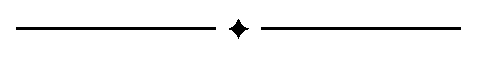
\includegraphics{diamondrule} is completely sufficient.
\graphicspath{{figs/}{figures/}{pictures/}{images/}{./}{template_ieee/}} % where to search for the images

%% Only used in the template examples. You can remove these lines.
\usepackage{tabu}                      % only used for the table example
\usepackage{booktabs}                  % only used for the table example
\usepackage{lipsum}                    % used to generate placeholder text
\usepackage{mwe}                       % used to generate placeholder figures

%% We encourage the use of mathptmx for consistent usage of times font
%% throughout the proceedings. However, if you encounter conflicts
%% with other math-related packages, you may want to disable it.
\usepackage{mathptmx}                  % use matching math font

%% ----------------- My Packages ----------------- %%

% To run some commands present in the .bib file
\usepackage{manfnt}

% Table from csv
\PassOptionsToPackage{svgnames}{xcolor}
\usepackage{pgfplotstable}
\pgfplotsset{compat=1.18}
\usepackage{multirow}
\usepackage{multicol}
\usepackage{soul}

% Author comments
\newcommand{\hsm}[1]{{\color{blue}{[H: #1]}}}
\newcommand{\fc}[1]{{\color{red}{[F: #1]}}}
\newcommand{\gv}[1]{{\color{orange}{[G: #1]}}}
\newcommand{\rs}[1]{{\color{green}{[R: #1]}}}
\newcommand{\al}[1]{{\color{violet}{[A: #1]}}}
\newcommand{\changed}[1]{{\color{magenta}{#1}}}

% Remove comments
\renewcommand{\hsm}[1]{}
\renewcommand{\fc}[1]{}
\renewcommand{\gv}[1]{}
\renewcommand{\rs}[1]{}
\renewcommand{\al}[1]{}
\renewcommand{\changed}[1]{#1}  % This will keep the changes but remove the color.


% Capitalize section autorefs
\newcommand\sectionautorefname{Section}

% SVG support
\usepackage{svg}

% Merge footnotes
% \usepackage{fixfoot}
% \DeclareFixedFootnote*{\hidden}{Citation hidden for double-blind review}
%% ----------------- End my Packages ----------------- %%

\begin{document}

\firstsection{Introduction}

\maketitle

%% \section{Introduction} %for journal use above \firstsection{..} instead
Virtual Reality (VR) technology has permeated numerous sectors beyond entertainment, becoming integral tools in fields such as healthcare, professional training, and education \cite{chatainGraspingDerivativesTeaching2022}.
Generally, VR is defined as a computer-generated simulation that enables users to perceive and interact with a three-dimensional environment through real-time multisensory feedback.
A typical VR system includes a head-mounted display for stereoscopic rendering, motion-tracked controllers or sensors for user input, and a computing unit for environment simulation and rendering.
However, there is no unifying definition of VR \cite{kardong-edgrenCallUnifyDefinitions2019}.

A barrier to widespread VR adoption is the onset of cybersickness (CS) \cite{casermanCybersicknessCurrentgenerationVirtual2021}.
Cybersickness is a form of visually induced motion sickness (VIMS) \cite{weechPresenceCybersicknessVirtual2019} characterized by symptoms such as nausea, dizziness, and disorientation that arise during or after immersion in a virtual environment \cite{casermanCybersicknessCurrentgenerationVirtual2021}.
The relationship between cybersickness, VIMS, simulator sickness, and motion sickness is treated in detail in Section~\ref{sec:theoretical}; the present review uses VIMS as the umbrella term when introducing constructs and uses the term each cited study employs when reporting its findings.
Cybersickness affects a substantial portion of the user population, with studies reporting prevalence between 60\% and 95\% \cite{casermanCybersicknessCurrentgenerationVirtual2021}, degrades user experience, impairs task performance, and can lead to premature session termination \cite{mimnaughVirtualRealitySickness2023}.

Assessment of cybersickness has historically relied on subjective post-hoc questionnaires such as the Simulator Sickness Questionnaire \cite{kennedySimulatorSicknessQuestionnaire1993}.
Such instruments are retrospective, prone to recall bias, and do not capture the dynamic nature of the experience \cite{changBrainActivityCybersickness2023, dennisonImprovingMotionSickness2019}.
This limitation creates a need for objective measures grounded in the user's physiology and for interventions that can modulate the user's state during exposure rather than after the fact.

Two converging lines of research have responded by examining the brain.
The first records neural activity --- primarily electroencephalography (EEG), and to a lesser extent functional near-infrared spectroscopy (fNIRS) --- to identify signals that index the onset, severity, or trajectory of cybersickness.
The second applies non-invasive brain stimulation, including galvanic vestibular stimulation (GVS), transcranial direct-current stimulation (tDCS), and transcranial alternating-current stimulation (tACS), to modulate the underlying processes that produce sickness.
We use the term \emph{neuromarkers} to refer to signals derived from either non-invasive recording or non-invasive modulation of brain activity in this context.
For a VR system designer, neuromarkers carry information that subjective questionnaires cannot: continuous, time-resolved indices of user state that can in principle drive adaptive content, comfort thresholds, and closed-loop mitigation.

Chang et al.~\cite{changBrainActivityCybersickness2023} synthesized 33 EEG studies published before September 2021 in a scoping review and characterized the EEG analysis pipeline used in cybersickness research.
The present systematic review differs in four respects.
First, the scope extends beyond EEG to include functional near-infrared spectroscopy and non-invasive neurostimulation, consistent with the integrated frame of neuromarkers.
Second, the corpus is larger and more recent: 92 studies retrieved up to 27~March~2025 from three curated databases (PubMed, Web of Science, Scopus), compared with 33 studies retrieved from Web of Science and Google Scholar up to September~2021.
Third, the synthesis includes corpus-level inferential statistics on hardware and methodological confounders, in addition to the pipeline characterization shared with prior work.
Fourth, this review situates the empirical findings within the broader context of the field: the theoretical frameworks invoked to explain cybersickness, the terminology used across the cybersickness, VIMS, simulator sickness, and motion sickness literatures, and a critical appraisal of recurring methodological shortcomings.
Where the prior scoping review concentrates on findings and pipelines, this review additionally examines the conceptual and methodological scaffolding in which those findings are produced.

The contributions of this review are threefold.
First, we provide a systematic synthesis of cybersickness neuromarkers in VR across 92 studies, covering neuroimaging and neurostimulation under a unified frame.
Second, we report meta-analytic evidence that VR display hardware significantly modulates the band-power response associated with cybersickness ($p=0.0036$ on alpha, large effect; $p=0.0146$ on beta), recasting prior contradictions in the EEG--cybersickness literature as partly attributable to hardware confounds rather than to differences in cybersickness per se.
Third, we conduct a methodological audit of the classification literature, finding that of 38 cybersickness classification or prediction studies, only one reports leave-one-subject-out validation, nineteen do not disclose a sick versus non-sick decision threshold, and thirteen report accuracy without sensitivity, specificity, AUC, or F1; we derive concrete reporting recommendations from these gaps for future VR-EEG and VR-stimulation work.
\TODO[intro]{Contributions are too narrow}

The remainder of this paper is organized as follows.
Section~\ref{sec:theoretical} reviews the relevant theoretical frameworks for cybersickness and the principal neuroimaging and stimulation modalities.
Section~\ref{sec:methodology} describes the review methodology and search strategy.
Section~\ref{sec:results} presents the corpus, the per-modality synthesis, and the corpus-level meta-analytic findings.
Section~\ref{sec:discussion} discusses methodological challenges and outlines future directions.
Section~\ref{sec:conclusion} concludes.

\section{Related Work}\label{sec:related-works}
\input{contents/related-work}

\section{Experiment}\label{sec:methods}
\input{contents/material-and-methods}

\section{Results}\label{sec:results}
The 92 corpus studies address four main research objectives: classification or prediction of cybersickness from physiological signals (38 studies), identification of neural and physiological correlates (24), development of mitigation strategies (18), and characterisation of individual susceptibility (3).
Nine residual studies (cognitive effects, recovery, dataset contributions, other framings) are integrated into the relevant subsections, with full discussion deferred to \autoref{sec:discussion}.
This section adds two cross-cutting layers on top of these objectives: \autoref{sec:corpus-characteristics} describes the corpus as a whole, and \autoref{sec:confounders} reports meta-analytic observations across the 92 studies.

Activity in the field has accelerated in recent years: 63.0\% of the corpus (58 of 92 studies) was published from 2021 onwards, with a corresponding shift toward classification, mitigation, and susceptibility objectives (\autoref{fig:stacked}).
Per-study sample sizes have also increased over the same period (Mann--Whitney $U$ on Recent versus Earlier studies, Cliff's $\delta = -0.308$, $p = 0.022$, medium effect).

\autoref{tab:all-studies} lists all 92 studies with their modality, sample size, virtual reality hardware, stimulus paradigm, cybersickness measure, primary objective, and topic.
% AUTO-GENERATED by review_scripts/analysis/emit_studies_table_latex.py
% Source: revision_notes/phase4/studies_table_final.csv
% Do not edit this file by hand; edit the source CSV and re-run the emitter.

\onecolumn
\begin{landscape}
\begin{footnotesize}
\setlength{\tabcolsep}{4pt}
\begin{longtable}{@{}p{1.0cm}>{\raggedright\arraybackslash}p{3.4cm}p{0.8cm}>{\raggedright\arraybackslash}p{2.0cm}>{\raggedright\arraybackslash}p{2.8cm}>{\raggedright\arraybackslash}p{1.6cm}>{\raggedright\arraybackslash}p{1.8cm}>{\raggedright\arraybackslash}p{8.0cm}@{}}
\caption{All 92 studies included in this systematic review. Modality: EEG, fNIRS, fMRI = neuroimaging; GVS = galvanic vestibular stimulation; tDCS/tACS = transcranial direct/alternating current stimulation; ECG, GSR, EOG, EMG, EGG = peripheral physiology; posturography = balance / centre-of-pressure recording. CS measure abbreviations: SSQ = Simulator Sickness Questionnaire; VRSQ = VR Sickness Questionnaire; FMS = Fast Motion-Sickness Scale; FMS+SSQ = repeated FMS sampling plus SSQ assessment; MSSQ = Motion Sickness Susceptibility Questionnaire; cont.\ = continuous self-report; Likert = single-item Likert; custom = study-specific scale; behav.\ = behavioural measure only; none = no cybersickness measure reported; studies listed as cont., Likert, or behav.\ without a named questionnaire did not report a specific instrument. Sample size N gives subjects analysed. Topic gives a short noun phrase describing the focus of each paper.}\label{tab:all-studies} \\
\toprule
\textbf{Ref.} & \textbf{Modality} & \textbf{N} & \textbf{VR device} & \textbf{Stimulus} & \textbf{CS measure} & \textbf{Objective} & \textbf{Topic} \\
\midrule
\endfirsthead

\multicolumn{8}{l}{\emph{Table \ref{tab:all-studies} continued from previous page}} \\
\toprule
\textbf{Ref.} & \textbf{Modality} & \textbf{N} & \textbf{VR device} & \textbf{Stimulus} & \textbf{CS measure} & \textbf{Objective} & \textbf{Topic} \\
\midrule
\endhead

\midrule
\multicolumn{8}{r}{\emph{Continued on next page}} \\
\endfoot

\bottomrule
\endlastfoot


\cite{abdalhadiDEVELOPMENTVIRTUALENVIRONMENT} & EEG & 2 & HMD & Mixed & none & Mitigation & EEG-informed scene-simplification mitigation \\
\cite{ahnTemporalDynamicsVisually2020} & EEG+\allowbreak{}EOG & 17 & HMD & Driving (passive) & SSQ & Correlates & Alpha connectivity and P3 in susceptibility \\
\cite{andrievskaiaExploringNeurophysiologicalCorrelates2023} & EEG+\allowbreak{}EOG & 33 & Screen & Passive viewing & FMS & Correlates & EEG time-frequency correlates of VIMS severity \\
\cite{argasinskiElectroencephalographicEEGCorrelates2023} & EEG & 31 & HMD & Mixed & SSQ & Correlates & Spectral EEG correlates of VIMS in HMD \\
\cite{balajiNeurodynamicMappingCybersickness2025} & EEG+\allowbreak{}ECG+\allowbreak{}GSR+\allowbreak{}EOG & 27 & HMD & Active navigation & custom & Classification & Spiking-network EEG+HRV cybersickness prediction \\
\cite{benelliFrequencyDependentReductionCybersickness2023} & tACS+\allowbreak{}GSR & 37 & HMD & Passive viewing & cont. & Mitigation & 10 Hz tACS over vestibular cortex \\
\cite{bergerSexDifferencesUser2021} & EEG & 68 & HMD & Mixed & SSQ & Other & Sex differences in EEG neurofeedback sessions \\
\cite{bergerInfluencePlaceboTDCS2024} & EEG+\allowbreak{}tDCS+\allowbreak{}ECG+\allowbreak{}EOG & 41 & HMD & Passive viewing & SSQ & Mitigation & Placebo tDCS in EEG neurofeedback for cybersickness \\
\cite{bergerManipulatingCybersicknessVirtual2025} & EEG+\allowbreak{}ECG & 39 & HMD & Active navigation & SSQ & Cognition & VR-parameter manipulation during EEG neurofeedback \\
\cite{chaiEEGStudyVirtual2023} & EEG & 15 & HMD & Passive viewing & SSQ & Classification & Resting-state EEG entropy classification \\
\cite{changEffectsRestFrames2013} & EEG & 12 & Screen & Passive viewing & SSQ & Mitigation & Rest-frame mitigation with EEG correlates \\
\cite{changIdentifyingPhysiologicalCorrelates2022} & EEG+\allowbreak{}ECG+\allowbreak{}EOG & 20 & Screen & Passive viewing & SSQ & Correlates & Heartbeat-evoked potentials as cybersickness correlates \\
\cite{chenMotionSicknessRelatedBrain2009} & EEG & 19 & Projector & Driving (passive) & cont. & Correlates & ICA-based motion sickness EEG component clusters \\
\cite{chenSpatialTemporalEEG2010} & EEG & 19 & Projector & Driving (passive) & cont. & Correlates & Continuous motion sickness EEG dynamics \\
\cite{chiossiMindVisualDiscomfort2024} & EEG & 20 & HMD & Other & SSQ & Correlates & blur-induced visual discomfort in HMDs \\
\cite{cortesEEGbasedExperimentVR2023} & EEG & 16 & HMD & Active navigation & SSQ & Correlates & EEG during VR sickness while walking \\
\cite{dasdemirClassificationEmotionalImmersive2023} & EEG & 32 & HMD & Mixed & SSQ & Dataset & EEG cybersickness dataset and benchmark \\
\cite{dasdemirLocomotionTechniquesEEG2023} & EEG & 32 & HMD & Active navigation & SSQ & Classification & EEG-based comparison of VR locomotion techniques \\
\cite{dennisonImprovingMotionSickness2019} & EEG+\allowbreak{}ECG+\allowbreak{}EOG+\allowbreak{}EGG+\allowbreak{}posturography & 20 & HMD & Active navigation & Likert & Classification & Multimodal EEG+physiology severity classification \\
\cite{emeksizConvolutionalTransformerModel2025} & EEG+\allowbreak{}ECG+\allowbreak{}GSR & 25 & Other & Passive viewing & SSQ & Classification & Convolutional-transformer EEG cybersickness detection \\
\cite{fengComprehensiveExplorationMotion2025} & EEG & 23 & HMD & Passive viewing & SSQ & Classification & Multi-domain EEG feature comparison \\
\cite{gallagherVectionVirtualReality2019} & EMG & 24 & HMD & Passive viewing & MSSQ & Correlates & VEMP changes after VR vection exposure \\
\cite{grothOmnidirectionalGalvanicVestibular2022a} & GVS & 47 & HMD & Passive viewing & SSQ & Mitigation & Omnidirectional GVS for 360° video viewing \\
\cite{huaAssessmentVirtualReality2023} & EEG+\allowbreak{}EOG & 23 & HMD & Passive viewing & SSQ & Classification & LSTM regression of continuous VRMS severity \\
\cite{huaEEGClassificationModel2024} & EEG & 15 & HMD & Mixed & SSQ & Classification & Multi-scale EEG brain-network classification \\
\cite{huaDetectionVirtualReality2024} & EEG & 15 & HMD & Passive viewing & SSQ & Classification & Bilateral asymmetry features for VRMS detection \\
\cite{huaSiamLSTMModelMultichannel2024} & EEG+\allowbreak{}EOG & 22 & HMD & Passive viewing & SSQ & Classification & Siam-LSTM with EEG functional brain networks \\
\cite{huaDualpathwayEEGModel2025} & EEG+\allowbreak{}posturography & 22 & HMD & Active navigation & VRSQ & Classification & Dual-pathway raw EEG and network model \\
\cite{jangEstimatingObjectiveEEG2022} & EEG & 40 & Screen & Passive viewing & SSQ & Indiv. diff. & EEG band-power correlates of cybersickness susceptibility \\
\cite{jeongCybersicknessAnalysisEEG2019} & EEG & 24 & HMD & Passive viewing & cont. & Classification & Deep-learning EEG classification of cybersickness \\
\cite{khaitamiEEGVisualizationCybersickness2019} & EEG & 9 & Screen & Active navigation & SSQ & Other & Gamma-band EEG visualisation of sickness onset \\
\cite{kimPsychophysiologicalChangesNavigation2001} & EEG+\allowbreak{}ECG+\allowbreak{}GSR+\allowbreak{}EOG & 45 & CAVE & Active navigation & SSQ & Correlates & EEG and autonomic correlates during navigation \\
\cite{kimCharacteristicChangesPhysiological2005} & EEG+\allowbreak{}ECG+\allowbreak{}GSR+\allowbreak{}EOG+\allowbreak{}EGG & 57 & Projector & Active navigation & SSQ & Correlates & Multimodal physiology of navigation cybersickness \\
\cite{kimDeepCybersicknessPredictor2019} & EEG & 202 & HMD & Passive viewing & Likert & Classification & EEG-to-video transfer for cybersickness prediction \\
\cite{kimPsychophysiologicalAlterationVirtual2019} & EEG+\allowbreak{}EOG & 30 & HMD & Passive viewing & SSQ & Correlates & Source-localised alpha cybersickness correlates after VR \\
\cite{koEstimatingLevelMotion2011} & EEG & 16 & Projector & Driving (passive) & cont. & Classification & ICA-EEG regression of motion-sickness level \\
\cite{koEEGbasedMotionSickness2013} & EEG & 6 & CAVE & Driving (passive) & cont. & Classification & Genetic feature selection for EEG classification \\
\cite{krokosQuantifyingVRCybersickness2022} & EEG & 43 & HMD & Passive viewing & cont. & Correlates & EEG band-power correlates with continuous joystick cybersickness \\
\cite{leeAssessingIndividualVR2022} & EEG+\allowbreak{}ECG+\allowbreak{}GSR & 40 & HMD; Screen & Passive viewing & SSQ & Classification & EEG and physiology fusion for SSQ estimation \\
\cite{liMachineLearningAssessment2019} & EEG+\allowbreak{}EOG+\allowbreak{}posturography & 20 & Projector & Driving (passive) & custom & Classification & Multimodal ensemble for VIMS severity \\
\cite{liVRMotionSickness2020} & EEG & 18 & HMD & Passive viewing & behav. & Classification & Wavelet-packet EEG features for VRMS \\
\cite{liExploringFeasibilityMitigating2020} & tDCS & 20 & HMD & Passive viewing & cont. & Mitigation & Cathodal parietal tDCS for cybersickness \\
\cite{liComparingAutonomicPhysiological2021} & EEG+\allowbreak{}EOG & 22 & HMD & Passive viewing & FMS & Classification & EEG vs. autonomic features for VR sickness \\
\cite{liExploringNeuralBiomarkers2023} & EEG+\allowbreak{}EOG & 20 & HMD & Passive viewing & FMS & Indiv. diff. & EEG biomarker of VRMS resistance \\
\cite{liRestingstateEEGVestibular2023} & EEG & 39 & HMD & Mixed & FMS & Classification & Resting EEG prediction of in-car VRMS \\
\cite{liReducedVRMotion2024} & EEG+\allowbreak{}tACS & 18 & HMD & Mixed & FMS & Mitigation & Online 18 Hz tACS over P3 \\
\cite{liaoUsingEEGDeep2020} & EEG & 130 & HMD & Passive viewing & custom & Classification & LSTM prediction of impending motion sickness \\
\cite{limTestretestReliabilityVirtual2021} & EEG & 16 & TV & Passive viewing & SSQ & Other & Test-retest reliability of EEG sickness markers \\
\cite{linEEGEffectsMotion2007} & EEG & 9 & Projector & Driving (passive) & custom & Correlates & EEG dynamics during VR motion sickness \\
\cite{linMotionSicknessEstimation2012} & EEG & 6 & CAVE & Driving (passive) & cont. & Classification & BCI estimation of motion-sickness level \\
\cite{lin653QuantizationCybersickness2018} & EEG+\allowbreak{}ECG & 25 & HMD & Passive viewing & cont. & Classification & Real-time EEG+ECG cybersickness warning \\
\cite{liuMeasuringVisuallyInduced2017} & EEG & 9 & CAVE & Driving (active) & cont. & Correlates & Wearable EEG and cardiovascular correlates \\
\cite{liuPilotStudyEEGBased2020} & EEG & 8 & Screen & Driving (active) & cont. & Correlates & Low-channel EEG markers for VIMS \\
\cite{liuExploringQuantitativeAssessment2024} & EEG & 36 & HMD & Passive viewing & SSQ & Classification & CNN-ECA-LSTM continuous cybersickness regression \\
\cite{liuExploringBrainPhysiological2024} & EEG & 36 & HMD & Passive viewing & SSQ & Classification & EEG spectral and network regression of severity \\
\cite{luoFeatureExtractionMethod2024} & EEG & 25 & HMD & Passive viewing & SSQ & Classification & Wavelet-packet GRU for VR motion sickness \\
\cite{mawalidClassificationEEGSignal2018} & EEG & 9 & Screen & Active navigation & SSQ & Classification & Time-domain EEG features for cybersickness \\
\cite{mimnaughVirtualRealitySickness2023} & EEG+\allowbreak{}EOG & 29 & HMD & Passive viewing & SSQ & Cognition & P3b ERP attention markers during VR sickness \\
\cite{moinnereauCybersicknessMarkerPrediction2024} & EEG+\allowbreak{}ECG+\allowbreak{}EOG & 8 & HMD & Active navigation & custom & Classification & Multimodal symptom-wise cybersickness markers \\
\cite{nakataExploringDisplayParameters2025} & EEG & 18 & HMD & Passive viewing & cont. & Correlates & EEG correlates of display-parameter cybersickness \\
\cite{namElectroencephalogramMicrostatesFunctional2022} & EEG & 40 & Screen & Passive viewing & SSQ & Correlates & EEG microstates and functional connectivity \\
\cite{nunesdasilvaAnalysisCybersicknessBiosignals2024} & ECG+\allowbreak{}GSR & 13 & HMD & Mixed & VRSQ & Classification & Symbolic ML on peripheral biosignals \\
\cite{nurnbergerMismatchVisualVestibularInformation2021} & EEG & 14 & HMD & Passive viewing & SSQ & Correlates & VIMS effective connectivity and predictive coding \\
\cite{ozkanEffectsSpeedComplexity2023} & EEG & 33 & HMD & Passive viewing & SSQ & Correlates & EEG across speed, complexity, and stereoscopy \\
\cite{paneIdentifyingSeverityLevel2018} & EEG & 9 & Screen & Active navigation & SSQ & Classification & Rule-based EEG severity classification \\
\cite{pradhanVisualVestibularConflict2022} & GVS+\allowbreak{}EGG & 19 & HMD & Active navigation & SSQ & Mitigation & Simulator-sickness GVS mitigation during flight VR \\
\cite{qiProfilingCybersicknessBalance2021} & GVS+\allowbreak{}balance & 140 & HMD & Passive viewing & custom & Correlates & GVS probing of vestibular contribution \\
\cite{recentiPredictingMotionSickness2021} & EEG+\allowbreak{}EMG & 28 & HMD & Passive viewing & MSSQ & Classification & BioVRSea EEG+EMG motion sickness prediction \\
\cite{rosannePreprocessNotPreprocess2025} & EEG+\allowbreak{}EOG & 20 & HMD & Mixed & FMS & Classification & EEG preprocessing trade-offs for cybersickness \\
\cite{sameriPhysiologydrivenCybersicknessDetection2024} & EEG+\allowbreak{}GSR & 22 & HMD & Passive viewing & SSQ & Classification & Explainable AI on multimodal physiology \\
\cite{shenClassificationVisuallyInduced2024} & EEG & 25 & HMD & Passive viewing & SSQ & Classification & PLV connectivity CNN-LSTM for VIMS \\
\cite{sraAddingProprioceptiveFeedback2019} & GVS+\allowbreak{}GSR & 20 & HMD & Passive viewing & SSQ & Mitigation & Wearable motion-synchronised GVS \\
\cite{suwandiElectroencephalographySignalAnalysis2023} & EEG & 22 & HMD; Screen & Passive viewing & SSQ & Correlates & EEG comparison of HMD versus screen VR \\
\cite{suwandiExploringImpactMotion2024} & EEG & 31 & HMD & Passive viewing & SSQ & Correlates & EEG across VR motion parameter variations \\
\cite{takeuchiModulationExcitabilityTemporoparietal2018} & tDCS+\allowbreak{}ECG+\allowbreak{}posturography & 20 & HMD & Passive viewing & SSQ & Mitigation & Anodal tDCS over right TPJ \\
\cite{tanimuraEffectsLowResolution3D2019} & fNIRS+\allowbreak{}ECG+\allowbreak{}posturography & 11 & HMD & Passive viewing & behav. & Correlates & fNIRS and posturography for 3D sickness \\
\cite{tianWhoSaysYou2024} & EEG+\allowbreak{}ECG+\allowbreak{}EGG & 28 & HMD & Mixed & FMS+SSQ & Indiv. diff. & EEG aperiodic activity for susceptibility profiling \\
\cite{uyanCDMSRealtimeSystem2024} & EEG & 53 & HMD & Passive viewing & SSQ & Mitigation & Real-time EEG-driven factor-specific mitigation \\
\cite{watanabeStudyVRSickness2025} & EEG & 6 & HMD & Active navigation & SSQ & Mitigation & Gaze-contingent peripheral blur mitigation \\
\cite{weechInfluenceBoneconductedVibration2018} & Other & 108 & Projector & Mixed & SSQ & Mitigation & Bone-conducted vibration vestibular stimulation \\
\cite{weechReductionCybersicknessImmediately2020} & GVS & 40 & HMD & Active navigation & FMS+SSQ & Mitigation & Noisy GVS for nauseogenic VR \\
\cite{weiEEGbasedEvaluationSystem2011} & EEG & 6 & Projector & Driving (passive) & cont. & Classification & Continuous EEG-based motion-sickness estimation \\
\cite{wooRecoveryTimeVR2023} & EEG & 40 & TV & Passive viewing & SSQ & Recovery & EEG recovery dynamics after VR exposure \\
\cite{wuInhibitionrelatedN2P32020} & EEG & 17 & HMD & Active navigation & SSQ & Cognition & Inhibition-related ERPs after VIMS \\
\cite{xuAssessingEffectsFullbody2019} & EEG & 12 & HMD & Other & SSQ & Cognition & Full-body exergame, simulator sickness, EEG theta \\
\cite{xuSECNNAttentionStructure2023} & EEG & 16 & HMD & Passive viewing & SSQ & Classification & SE-CNN regression of VR motion sickness from EEG \\
\cite{yamamuraPleasantLocomotionReducing2020} & fNIRS & 1 & HMD & Active navigation & SSQ & Mitigation & fNIRS-triggered FOV-narrowing mitigation \\
\cite{yamamuraHemodynamicVRAdaptingUsers2021} & fNIRS & 10 & HMD & Mixed & SSQ & Mitigation & Wearable fNIRS for adaptive FOV restriction \\
\cite{yangPredictionDetectionVirtual2023} & EEG+\allowbreak{}ECG & 64 & HMD & Passive viewing & SSQ & Classification & Interpretable spiking-network EEG prediction \\
\cite{yeoEEGbasedAnalysisVarious2022} & EEG & 25 & HMD & Mixed & FMS+SSQ & Mitigation & Multisensory VIMS mitigation with EEG correlates \\
\cite{yeoInvestigatingCorticalActivity2024} & fNIRS & 30 & HMD & Passive viewing & SSQ & Correlates & fNIRS angular-gyrus correlates of cybersickness \\
\cite{zhouApplicationEEGSTransformation2023} & EEG+\allowbreak{}EOG & 15 & HMD & Passive viewing & none & Classification & S-transform EEG features for cybersickness \\

\end{longtable}
\end{footnotesize}
\end{landscape}
\twocolumn




\begin{figure}[t]
    \centering
    
\includegraphics[width=\linewidth]{figures/year_objective_stacked.pdf}
    \caption{Distribution of reviewed papers by year and primary research objective.}
    \label{fig:stacked}
\end{figure}

The remainder of this section synthesises findings thematically along the axes above.

%%%%%%%%%%%%%%%%%%%%%%%%%           Corpus characteristics          %%%%%%%%%%%%%%%%%%%%%%%%%%%%%

\subsection{Corpus Characteristics}\label{sec:corpus-characteristics}

The 92 included studies cluster on EEG-based investigations of young adults in head-mounted VR, but vary widely on baseline condition, montage, and preprocessing.
The dispersion documented in this subsection is the precondition for the meta-analytic observations reported in \autoref{sec:confounders}.

\subsubsection{Sample Sizes and Demographics}
The 92 studies span 2001--2025.
Across the corpus, 2687 participants were analysed (recruited: 2822), with a mean of 29.2 $\pm$ 29.0 participants analysed per study (median: 22, range: 1--202).
The 62 studies that report a parsable adult-age range yield a mean age of 23.7 $\pm$ 2.7 years, indicating a focus on young-adult populations; 14 studies do not report age or report ranges that cannot be parsed (\autoref{fig:age_distribution}).

\begin{figure}[htbp]
\centering
\begin{tikzpicture}
\begin{axis}[
    width=\columnwidth,
    height=0.6\textheight,
    xlabel={Age (years)},
    ylabel={Studies},
    grid=major,
    grid style={dashed,gray!30},
    tick style={font=\footnotesize},
    label style={font=\small},
    title style={font=\normalsize},
    title={Age Distribution: Range and Standard Deviation},
    ytick={0,1,2,3,4,5,6,7,8,9,10,11,12,13,14,15,16,17,18,19,20,21,22,23,24,25,26,27,28,29,30,31,32,33,34,35,36,37,38,39,40,41,42,43,44,45,46,47,48,49,50,51,52,53,54,55,56,57,58,59,60,61},
    yticklabels={\cite{liaoUsingEEGDeep2020},\cite{weechInfluenceBoneconductedVibration2018},\cite{huaDetectionVirtualReality2024},\cite{nakataExploringDisplayParameters2025},\cite{zhouApplicationEEGSTransformation2023},\cite{chaiEEGStudyVirtual2023},\cite{qiProfilingCybersicknessBalance2021},\cite{gallagherVectionVirtualReality2019},\cite{liExploringFeasibilityMitigating2020},\cite{shenClassificationVisuallyInduced2024},\cite{dasdemirClassificationEmotionalImmersive2023},\cite{dasdemirLocomotionTechniquesEEG2023},\cite{takeuchiModulationExcitabilityTemporoparietal2018},\cite{lin653QuantizationCybersickness2018},\cite{weechReductionCybersicknessImmediately2020},\cite{huaEEGClassificationModel2024},\cite{linEEGEffectsMotion2007},\cite{liExploringNeuralBiomarkers2023},\cite{chenSpatialTemporalEEG2010},\cite{chenMotionSicknessRelatedBrain2009},\cite{xuAssessingEffectsFullbody2019},\cite{tanimuraEffectsLowResolution3D2019},\cite{fengComprehensiveExplorationMotion2025},\cite{huaAssessmentVirtualReality2023},\cite{huaSiamLSTMModelMultichannel2024},\cite{liMachineLearningAssessment2019},\cite{yangPredictionDetectionVirtual2023},\cite{kimCharacteristicChangesPhysiological2005},\cite{mimnaughVirtualRealitySickness2023},\cite{bergerSexDifferencesUser2021},\cite{tianWhoSaysYou2024},\cite{recentiPredictingMotionSickness2021},\cite{ozkanEffectsSpeedComplexity2023},\cite{changEffectsRestFrames2013},\cite{bergerInfluencePlaceboTDCS2024},\cite{jangEstimatingObjectiveEEG2022},\cite{namElectroencephalogramMicrostatesFunctional2022},\cite{wooRecoveryTimeVR2023},\cite{yeoEEGbasedAnalysisVarious2022},\cite{yeoInvestigatingCorticalActivity2024},\cite{yamamuraHemodynamicVRAdaptingUsers2021},\cite{changIdentifyingPhysiologicalCorrelates2022},\cite{grothOmnidirectionalGalvanicVestibular2022a},\cite{liuExploringQuantitativeAssessment2024},\cite{liuExploringBrainPhysiological2024},\cite{limTestretestReliabilityVirtual2021},\cite{kimPsychophysiologicalAlterationVirtual2019},\cite{khaitamiEEGVisualizationCybersickness2019},\cite{uyanCDMSRealtimeSystem2024},\cite{chiossiMindVisualDiscomfort2024},\cite{cortesEEGbasedExperimentVR2023},\cite{wuInhibitionrelatedN2P32020},\cite{benelliFrequencyDependentReductionCybersickness2023},\cite{andrievskaiaExploringNeurophysiologicalCorrelates2023},\cite{krokosQuantifyingVRCybersickness2022},\cite{abdalhadiDEVELOPMENTVIRTUALENVIRONMENT},\cite{argasinskiElectroencephalographicEEGCorrelates2023},\cite{nurnbergerMismatchVisualVestibularInformation2021},\cite{moinnereauCybersicknessMarkerPrediction2024},\cite{liVRMotionSickness2020},\cite{ahnTemporalDynamicsVisually2020},\cite{pradhanVisualVestibularConflict2022}},
    yticklabel style={font=\tiny},
    xmin=3.5,
    xmax=58.5,
    enlarge y limits=0.05,
    legend pos=south east,
    legend style={font=\tiny},
]

% Mean points
\addplot[only marks, mark=*, mark size=2pt, black] coordinates {
    (16.54, 0)
    (18.63, 1)
    (20.4, 2)
    (20.4, 3)
    (20.4, 4)
    (20.4, 5)
    (21.05, 6)
    (21.13, 7)
    (21.2, 8)
    (21.32, 9)
    (21.44, 10)
    (21.44, 11)
    (21.5, 12)
    (21.96, 13)
    (22.0, 14)
    (22.0, 15)
    (22.0, 16)
    (22.0, 17)
    (22.1, 18)
    (22.1, 19)
    (22.42, 20)
    (22.6, 21)
    (22.8, 22)
    (22.8, 23)
    (22.8, 24)
    (22.8, 25)
    (23.0, 26)
    (23.08, 27)
    (23.11, 28)
    (23.21, 29)
    (23.3, 30)
    (23.8, 31)
    (23.8, 32)
    (23.91, 33)
    (23.95, 34)
    (23.95, 35)
    (24.1, 36)
    (24.1, 37)
    (24.12, 38)
    (24.17, 39)
    (24.2, 40)
    (24.65, 41)
    (24.79, 42)
    (24.8, 43)
    (24.8, 44)
    (25.0, 45)
    (25.0, 46)
    (25.11, 47)
    (25.4, 48)
    (25.4, 49)
    (25.73, 50)
    (25.8, 51)
    (26.3, 52)
    (26.7, 53)
    (27.0, 54)
    (28.0, 55)
    (28.1, 56)
    (28.8, 57)
    (28.9, 58)
    (29.3, 59)
    (29.7, 60)
    (31.0, 61)
};
\addlegendentry{Mean age}

% Age range error bars (min-max)
\draw[black, line width=1.0pt, densely dotted] (axis cs:6.0,0) -- (axis cs:23.0,0);
\draw[black, line width=1.0pt] (axis cs:6.0,-0.15) -- (axis cs:6.0,0.15);
\draw[black, line width=1.0pt] (axis cs:23.0,-0.15) -- (axis cs:23.0,0.15);
\draw[black, line width=1.0pt, densely dotted] (axis cs:17.0,1) -- (axis cs:27.0,1);
\draw[black, line width=1.0pt] (axis cs:17.0,0.85) -- (axis cs:17.0,1.15);
\draw[black, line width=1.0pt] (axis cs:27.0,0.85) -- (axis cs:27.0,1.15);
\draw[black, line width=1.0pt, densely dotted] (axis cs:18.0,10) -- (axis cs:30.0,10);
\draw[black, line width=1.0pt] (axis cs:18.0,9.85) -- (axis cs:18.0,10.15);
\draw[black, line width=1.0pt] (axis cs:30.0,9.85) -- (axis cs:30.0,10.15);
\draw[black, line width=1.0pt, densely dotted] (axis cs:18.0,11) -- (axis cs:30.0,11);
\draw[black, line width=1.0pt] (axis cs:18.0,10.85) -- (axis cs:18.0,11.15);
\draw[black, line width=1.0pt] (axis cs:30.0,10.85) -- (axis cs:30.0,11.15);
\draw[black, line width=1.0pt, densely dotted] (axis cs:20.0,12) -- (axis cs:24.0,12);
\draw[black, line width=1.0pt] (axis cs:20.0,11.85) -- (axis cs:20.0,12.15);
\draw[black, line width=1.0pt] (axis cs:24.0,11.85) -- (axis cs:24.0,12.15);
\draw[black, line width=1.0pt, densely dotted] (axis cs:20.0,13) -- (axis cs:31.0,13);
\draw[black, line width=1.0pt] (axis cs:20.0,12.85) -- (axis cs:20.0,13.15);
\draw[black, line width=1.0pt] (axis cs:31.0,12.85) -- (axis cs:31.0,13.15);
\draw[black, line width=1.0pt, densely dotted] (axis cs:18.0,14) -- (axis cs:56.0,14);
\draw[black, line width=1.0pt] (axis cs:18.0,13.85) -- (axis cs:18.0,14.15);
\draw[black, line width=1.0pt] (axis cs:56.0,13.85) -- (axis cs:56.0,14.15);
\draw[black, line width=1.0pt, densely dotted] (axis cs:19.0,15) -- (axis cs:25.0,15);
\draw[black, line width=1.0pt] (axis cs:19.0,14.85) -- (axis cs:19.0,15.15);
\draw[black, line width=1.0pt] (axis cs:25.0,14.85) -- (axis cs:25.0,15.15);
\draw[black, line width=1.0pt, densely dotted] (axis cs:18.0,16) -- (axis cs:26.0,16);
\draw[black, line width=1.0pt] (axis cs:18.0,15.85) -- (axis cs:18.0,16.15);
\draw[black, line width=1.0pt] (axis cs:26.0,15.85) -- (axis cs:26.0,16.15);
\draw[black, line width=1.0pt, densely dotted] (axis cs:20.0,17) -- (axis cs:32.0,17);
\draw[black, line width=1.0pt] (axis cs:20.0,16.85) -- (axis cs:20.0,17.15);
\draw[black, line width=1.0pt] (axis cs:32.0,16.85) -- (axis cs:32.0,17.15);
\draw[black, line width=1.0pt, densely dotted] (axis cs:21.0,18) -- (axis cs:24.0,18);
\draw[black, line width=1.0pt] (axis cs:21.0,17.85) -- (axis cs:21.0,18.15);
\draw[black, line width=1.0pt] (axis cs:24.0,17.85) -- (axis cs:24.0,18.15);
\draw[black, line width=1.0pt, densely dotted] (axis cs:21.0,19) -- (axis cs:24.0,19);
\draw[black, line width=1.0pt] (axis cs:21.0,18.85) -- (axis cs:21.0,19.15);
\draw[black, line width=1.0pt] (axis cs:24.0,18.85) -- (axis cs:24.0,19.15);
\draw[black, line width=1.0pt, densely dotted] (axis cs:19.0,20) -- (axis cs:29.0,20);
\draw[black, line width=1.0pt] (axis cs:19.0,19.85) -- (axis cs:19.0,20.15);
\draw[black, line width=1.0pt] (axis cs:29.0,19.85) -- (axis cs:29.0,20.15);
\draw[black, line width=1.0pt, densely dotted] (axis cs:18.0,25) -- (axis cs:27.0,25);
\draw[black, line width=1.0pt] (axis cs:18.0,24.85) -- (axis cs:18.0,25.15);
\draw[black, line width=1.0pt] (axis cs:27.0,24.85) -- (axis cs:27.0,25.15);
\draw[black, line width=1.0pt, densely dotted] (axis cs:18.0,26) -- (axis cs:33.0,26);
\draw[black, line width=1.0pt] (axis cs:18.0,25.85) -- (axis cs:18.0,26.15);
\draw[black, line width=1.0pt] (axis cs:33.0,25.85) -- (axis cs:33.0,26.15);
\draw[black, line width=1.0pt, densely dotted] (axis cs:19.0,27) -- (axis cs:27.0,27);
\draw[black, line width=1.0pt] (axis cs:19.0,26.85) -- (axis cs:19.0,27.15);
\draw[black, line width=1.0pt] (axis cs:27.0,26.85) -- (axis cs:27.0,27.15);
\draw[black, line width=1.0pt, densely dotted] (axis cs:18.0,28) -- (axis cs:50.0,28);
\draw[black, line width=1.0pt] (axis cs:18.0,27.85) -- (axis cs:18.0,28.15);
\draw[black, line width=1.0pt] (axis cs:50.0,27.85) -- (axis cs:50.0,28.15);
\draw[black, line width=1.0pt, densely dotted] (axis cs:18.0,29) -- (axis cs:34.0,29);
\draw[black, line width=1.0pt] (axis cs:18.0,28.85) -- (axis cs:18.0,29.15);
\draw[black, line width=1.0pt] (axis cs:34.0,28.85) -- (axis cs:34.0,29.15);
\draw[black, line width=1.0pt, densely dotted] (axis cs:20.0,30) -- (axis cs:45.0,30);
\draw[black, line width=1.0pt] (axis cs:20.0,29.85) -- (axis cs:20.0,30.15);
\draw[black, line width=1.0pt] (axis cs:45.0,29.85) -- (axis cs:45.0,30.15);
\draw[black, line width=1.0pt, densely dotted] (axis cs:18.0,32) -- (axis cs:42.0,32);
\draw[black, line width=1.0pt] (axis cs:18.0,31.85) -- (axis cs:18.0,32.15);
\draw[black, line width=1.0pt] (axis cs:42.0,31.85) -- (axis cs:42.0,32.15);
\draw[black, line width=1.0pt, densely dotted] (axis cs:18.0,34) -- (axis cs:34.0,34);
\draw[black, line width=1.0pt] (axis cs:18.0,33.85) -- (axis cs:18.0,34.15);
\draw[black, line width=1.0pt] (axis cs:34.0,33.85) -- (axis cs:34.0,34.15);
\draw[black, line width=1.0pt, densely dotted] (axis cs:19.0,42) -- (axis cs:52.0,42);
\draw[black, line width=1.0pt] (axis cs:19.0,41.85) -- (axis cs:19.0,42.15);
\draw[black, line width=1.0pt] (axis cs:52.0,41.85) -- (axis cs:52.0,42.15);
\draw[black, line width=1.0pt, densely dotted] (axis cs:20.0,46) -- (axis cs:37.0,46);
\draw[black, line width=1.0pt] (axis cs:20.0,45.85) -- (axis cs:20.0,46.15);
\draw[black, line width=1.0pt] (axis cs:37.0,45.85) -- (axis cs:37.0,46.15);
\draw[black, line width=1.0pt, densely dotted] (axis cs:19.0,47) -- (axis cs:30.0,47);
\draw[black, line width=1.0pt] (axis cs:19.0,46.85) -- (axis cs:19.0,47.15);
\draw[black, line width=1.0pt] (axis cs:30.0,46.85) -- (axis cs:30.0,47.15);
\draw[black, line width=1.0pt, densely dotted] (axis cs:18.0,48) -- (axis cs:42.0,48);
\draw[black, line width=1.0pt] (axis cs:18.0,47.85) -- (axis cs:18.0,48.15);
\draw[black, line width=1.0pt] (axis cs:42.0,47.85) -- (axis cs:42.0,48.15);
\draw[black, line width=1.0pt, densely dotted] (axis cs:19.0,53) -- (axis cs:44.0,53);
\draw[black, line width=1.0pt] (axis cs:19.0,52.85) -- (axis cs:19.0,53.15);
\draw[black, line width=1.0pt] (axis cs:44.0,52.85) -- (axis cs:44.0,53.15);
\draw[black, line width=1.0pt, densely dotted] (axis cs:18.0,56) -- (axis cs:42.0,56);
\draw[black, line width=1.0pt] (axis cs:18.0,55.85) -- (axis cs:18.0,56.15);
\draw[black, line width=1.0pt] (axis cs:42.0,55.85) -- (axis cs:42.0,56.15);
\draw[black, line width=1.0pt, densely dotted] (axis cs:23.0,57) -- (axis cs:37.0,57);
\draw[black, line width=1.0pt] (axis cs:23.0,56.85) -- (axis cs:23.0,57.15);
\draw[black, line width=1.0pt] (axis cs:37.0,56.85) -- (axis cs:37.0,57.15);
\draw[black, line width=1.0pt, densely dotted] (axis cs:21.0,60) -- (axis cs:48.0,60);
\draw[black, line width=1.0pt] (axis cs:21.0,59.85) -- (axis cs:21.0,60.15);
\draw[black, line width=1.0pt] (axis cs:48.0,59.85) -- (axis cs:48.0,60.15);

% Standard deviation error bars (mean ± std)
\draw[gray, line width=1.0pt] (axis cs:14.37,0) -- (axis cs:18.71,0);
\draw[gray, line width=1.0pt] (axis cs:14.37,-0.1) -- (axis cs:14.37,0.1);
\draw[gray, line width=1.0pt] (axis cs:18.71,-0.1) -- (axis cs:18.71,0.1);
\draw[gray, line width=1.0pt] (axis cs:17.11,1) -- (axis cs:20.15,1);
\draw[gray, line width=1.0pt] (axis cs:17.11,0.9) -- (axis cs:17.11,1.1);
\draw[gray, line width=1.0pt] (axis cs:20.15,0.9) -- (axis cs:20.15,1.1);
\draw[gray, line width=1.0pt] (axis cs:18.9,2) -- (axis cs:21.9,2);
\draw[gray, line width=1.0pt] (axis cs:18.9,1.9) -- (axis cs:18.9,2.1);
\draw[gray, line width=1.0pt] (axis cs:21.9,1.9) -- (axis cs:21.9,2.1);
\draw[gray, line width=1.0pt] (axis cs:18.4,3) -- (axis cs:22.4,3);
\draw[gray, line width=1.0pt] (axis cs:18.4,2.9) -- (axis cs:18.4,3.1);
\draw[gray, line width=1.0pt] (axis cs:22.4,2.9) -- (axis cs:22.4,3.1);
\draw[gray, line width=1.0pt] (axis cs:18.9,4) -- (axis cs:21.9,4);
\draw[gray, line width=1.0pt] (axis cs:18.9,3.9) -- (axis cs:18.9,4.1);
\draw[gray, line width=1.0pt] (axis cs:21.9,3.9) -- (axis cs:21.9,4.1);
\draw[gray, line width=1.0pt] (axis cs:18.9,5) -- (axis cs:21.9,5);
\draw[gray, line width=1.0pt] (axis cs:18.9,4.9) -- (axis cs:18.9,5.1);
\draw[gray, line width=1.0pt] (axis cs:21.9,4.9) -- (axis cs:21.9,5.1);
\draw[gray, line width=1.0pt] (axis cs:19.080000000000002,6) -- (axis cs:23.02,6);
\draw[gray, line width=1.0pt] (axis cs:19.080000000000002,5.9) -- (axis cs:19.080000000000002,6.1);
\draw[gray, line width=1.0pt] (axis cs:23.02,5.9) -- (axis cs:23.02,6.1);
\draw[gray, line width=1.0pt] (axis cs:17.23,7) -- (axis cs:25.029999999999998,7);
\draw[gray, line width=1.0pt] (axis cs:17.23,6.9) -- (axis cs:17.23,7.1);
\draw[gray, line width=1.0pt] (axis cs:25.029999999999998,6.9) -- (axis cs:25.029999999999998,7.1);
\draw[gray, line width=1.0pt] (axis cs:19.05,9) -- (axis cs:23.59,9);
\draw[gray, line width=1.0pt] (axis cs:19.05,8.9) -- (axis cs:19.05,9.1);
\draw[gray, line width=1.0pt] (axis cs:23.59,8.9) -- (axis cs:23.59,9.1);
\draw[gray, line width=1.0pt] (axis cs:19.32,10) -- (axis cs:23.560000000000002,10);
\draw[gray, line width=1.0pt] (axis cs:19.32,9.9) -- (axis cs:19.32,10.1);
\draw[gray, line width=1.0pt] (axis cs:23.560000000000002,9.9) -- (axis cs:23.560000000000002,10.1);
\draw[gray, line width=1.0pt] (axis cs:19.32,11) -- (axis cs:23.560000000000002,11);
\draw[gray, line width=1.0pt] (axis cs:19.32,10.9) -- (axis cs:19.32,11.1);
\draw[gray, line width=1.0pt] (axis cs:23.560000000000002,10.9) -- (axis cs:23.560000000000002,11.1);
\draw[gray, line width=1.0pt] (axis cs:20.4,12) -- (axis cs:22.6,12);
\draw[gray, line width=1.0pt] (axis cs:20.4,11.9) -- (axis cs:20.4,12.1);
\draw[gray, line width=1.0pt] (axis cs:22.6,11.9) -- (axis cs:22.6,12.1);
\draw[gray, line width=1.0pt] (axis cs:19.69,13) -- (axis cs:24.23,13);
\draw[gray, line width=1.0pt] (axis cs:19.69,12.9) -- (axis cs:19.69,13.1);
\draw[gray, line width=1.0pt] (axis cs:24.23,12.9) -- (axis cs:24.23,13.1);
\draw[gray, line width=1.0pt] (axis cs:14.96,14) -- (axis cs:29.04,14);
\draw[gray, line width=1.0pt] (axis cs:14.96,13.9) -- (axis cs:14.96,14.1);
\draw[gray, line width=1.0pt] (axis cs:29.04,13.9) -- (axis cs:29.04,14.1);
\draw[gray, line width=1.0pt] (axis cs:21.6,21) -- (axis cs:23.6,21);
\draw[gray, line width=1.0pt] (axis cs:21.6,20.9) -- (axis cs:21.6,21.1);
\draw[gray, line width=1.0pt] (axis cs:23.6,20.9) -- (axis cs:23.6,21.1);
\draw[gray, line width=1.0pt] (axis cs:21.7,22) -- (axis cs:23.900000000000002,22);
\draw[gray, line width=1.0pt] (axis cs:21.7,21.9) -- (axis cs:21.7,22.1);
\draw[gray, line width=1.0pt] (axis cs:23.900000000000002,21.9) -- (axis cs:23.900000000000002,22.1);
\draw[gray, line width=1.0pt] (axis cs:21.7,23) -- (axis cs:23.900000000000002,23);
\draw[gray, line width=1.0pt] (axis cs:21.7,22.9) -- (axis cs:21.7,23.1);
\draw[gray, line width=1.0pt] (axis cs:23.900000000000002,22.9) -- (axis cs:23.900000000000002,23.1);
\draw[gray, line width=1.0pt] (axis cs:21.7,24) -- (axis cs:23.900000000000002,24);
\draw[gray, line width=1.0pt] (axis cs:21.7,23.9) -- (axis cs:21.7,24.1);
\draw[gray, line width=1.0pt] (axis cs:23.900000000000002,23.9) -- (axis cs:23.900000000000002,24.1);
\draw[gray, line width=1.0pt] (axis cs:18.9,26) -- (axis cs:27.1,26);
\draw[gray, line width=1.0pt] (axis cs:18.9,25.9) -- (axis cs:18.9,26.1);
\draw[gray, line width=1.0pt] (axis cs:27.1,25.9) -- (axis cs:27.1,26.1);
\draw[gray, line width=1.0pt] (axis cs:21.029999999999998,27) -- (axis cs:25.13,27);
\draw[gray, line width=1.0pt] (axis cs:21.029999999999998,26.9) -- (axis cs:21.029999999999998,27.1);
\draw[gray, line width=1.0pt] (axis cs:25.13,26.9) -- (axis cs:25.13,27.1);
\draw[gray, line width=1.0pt] (axis cs:16.24,28) -- (axis cs:29.98,28);
\draw[gray, line width=1.0pt] (axis cs:16.24,27.9) -- (axis cs:16.24,28.1);
\draw[gray, line width=1.0pt] (axis cs:29.98,27.9) -- (axis cs:29.98,28.1);
\draw[gray, line width=1.0pt] (axis cs:19.8,29) -- (axis cs:26.62,29);
\draw[gray, line width=1.0pt] (axis cs:19.8,28.9) -- (axis cs:19.8,29.1);
\draw[gray, line width=1.0pt] (axis cs:26.62,28.9) -- (axis cs:26.62,29.1);
\draw[gray, line width=1.0pt] (axis cs:18.9,30) -- (axis cs:27.700000000000003,30);
\draw[gray, line width=1.0pt] (axis cs:18.9,29.9) -- (axis cs:18.9,30.1);
\draw[gray, line width=1.0pt] (axis cs:27.700000000000003,29.9) -- (axis cs:27.700000000000003,30.1);
\draw[gray, line width=1.0pt] (axis cs:22.6,31) -- (axis cs:25.0,31);
\draw[gray, line width=1.0pt] (axis cs:22.6,30.9) -- (axis cs:22.6,31.1);
\draw[gray, line width=1.0pt] (axis cs:25.0,30.9) -- (axis cs:25.0,31.1);
\draw[gray, line width=1.0pt] (axis cs:18.240000000000002,32) -- (axis cs:29.36,32);
\draw[gray, line width=1.0pt] (axis cs:18.240000000000002,31.9) -- (axis cs:18.240000000000002,32.1);
\draw[gray, line width=1.0pt] (axis cs:29.36,31.9) -- (axis cs:29.36,32.1);
\draw[gray, line width=1.0pt] (axis cs:22.03,33) -- (axis cs:25.79,33);
\draw[gray, line width=1.0pt] (axis cs:22.03,32.9) -- (axis cs:22.03,33.1);
\draw[gray, line width=1.0pt] (axis cs:25.79,32.9) -- (axis cs:25.79,33.1);
\draw[gray, line width=1.0pt] (axis cs:21.99,35) -- (axis cs:25.91,35);
\draw[gray, line width=1.0pt] (axis cs:21.99,34.9) -- (axis cs:21.99,35.1);
\draw[gray, line width=1.0pt] (axis cs:25.91,34.9) -- (axis cs:25.91,35.1);
\draw[gray, line width=1.0pt] (axis cs:21.8,36) -- (axis cs:26.400000000000002,36);
\draw[gray, line width=1.0pt] (axis cs:21.8,35.9) -- (axis cs:21.8,36.1);
\draw[gray, line width=1.0pt] (axis cs:26.400000000000002,35.9) -- (axis cs:26.400000000000002,36.1);
\draw[gray, line width=1.0pt] (axis cs:21.8,37) -- (axis cs:26.400000000000002,37);
\draw[gray, line width=1.0pt] (axis cs:21.8,36.9) -- (axis cs:21.8,37.1);
\draw[gray, line width=1.0pt] (axis cs:26.400000000000002,36.9) -- (axis cs:26.400000000000002,37.1);
\draw[gray, line width=1.0pt] (axis cs:21.32,38) -- (axis cs:26.92,38);
\draw[gray, line width=1.0pt] (axis cs:21.32,37.9) -- (axis cs:21.32,38.1);
\draw[gray, line width=1.0pt] (axis cs:26.92,37.9) -- (axis cs:26.92,38.1);
\draw[gray, line width=1.0pt] (axis cs:20.8,39) -- (axis cs:27.540000000000003,39);
\draw[gray, line width=1.0pt] (axis cs:20.8,38.9) -- (axis cs:20.8,39.1);
\draw[gray, line width=1.0pt] (axis cs:27.540000000000003,38.9) -- (axis cs:27.540000000000003,39.1);
\draw[gray, line width=1.0pt] (axis cs:22.869999999999997,40) -- (axis cs:25.53,40);
\draw[gray, line width=1.0pt] (axis cs:22.869999999999997,39.9) -- (axis cs:22.869999999999997,40.1);
\draw[gray, line width=1.0pt] (axis cs:25.53,39.9) -- (axis cs:25.53,40.1);
\draw[gray, line width=1.0pt] (axis cs:22.169999999999998,41) -- (axis cs:27.13,41);
\draw[gray, line width=1.0pt] (axis cs:22.169999999999998,40.9) -- (axis cs:22.169999999999998,41.1);
\draw[gray, line width=1.0pt] (axis cs:27.13,40.9) -- (axis cs:27.13,41.1);
\draw[gray, line width=1.0pt] (axis cs:19.07,42) -- (axis cs:30.509999999999998,42);
\draw[gray, line width=1.0pt] (axis cs:19.07,41.9) -- (axis cs:19.07,42.1);
\draw[gray, line width=1.0pt] (axis cs:30.509999999999998,41.9) -- (axis cs:30.509999999999998,42.1);
\draw[gray, line width=1.0pt] (axis cs:21.2,43) -- (axis cs:28.400000000000002,43);
\draw[gray, line width=1.0pt] (axis cs:21.2,42.9) -- (axis cs:21.2,43.1);
\draw[gray, line width=1.0pt] (axis cs:28.400000000000002,42.9) -- (axis cs:28.400000000000002,43.1);
\draw[gray, line width=1.0pt] (axis cs:21.2,44) -- (axis cs:28.400000000000002,44);
\draw[gray, line width=1.0pt] (axis cs:21.2,43.9) -- (axis cs:21.2,44.1);
\draw[gray, line width=1.0pt] (axis cs:28.400000000000002,43.9) -- (axis cs:28.400000000000002,44.1);
\draw[gray, line width=1.0pt] (axis cs:22.8,45) -- (axis cs:27.2,45);
\draw[gray, line width=1.0pt] (axis cs:22.8,44.9) -- (axis cs:22.8,45.1);
\draw[gray, line width=1.0pt] (axis cs:27.2,44.9) -- (axis cs:27.2,45.1);
\draw[gray, line width=1.0pt] (axis cs:21.0,46) -- (axis cs:29.0,46);
\draw[gray, line width=1.0pt] (axis cs:21.0,45.9) -- (axis cs:21.0,46.1);
\draw[gray, line width=1.0pt] (axis cs:29.0,45.9) -- (axis cs:29.0,46.1);
\draw[gray, line width=1.0pt] (axis cs:20.599999999999998,49) -- (axis cs:30.2,49);
\draw[gray, line width=1.0pt] (axis cs:20.599999999999998,48.9) -- (axis cs:20.599999999999998,49.1);
\draw[gray, line width=1.0pt] (axis cs:30.2,48.9) -- (axis cs:30.2,49.1);
\draw[gray, line width=1.0pt] (axis cs:22.13,50) -- (axis cs:29.330000000000002,50);
\draw[gray, line width=1.0pt] (axis cs:22.13,49.9) -- (axis cs:22.13,50.1);
\draw[gray, line width=1.0pt] (axis cs:29.330000000000002,49.9) -- (axis cs:29.330000000000002,50.1);
\draw[gray, line width=1.0pt] (axis cs:23.900000000000002,51) -- (axis cs:27.7,51);
\draw[gray, line width=1.0pt] (axis cs:23.900000000000002,50.9) -- (axis cs:23.900000000000002,51.1);
\draw[gray, line width=1.0pt] (axis cs:27.7,50.9) -- (axis cs:27.7,51.1);
\draw[gray, line width=1.0pt] (axis cs:23.5,52) -- (axis cs:29.1,52);
\draw[gray, line width=1.0pt] (axis cs:23.5,51.9) -- (axis cs:23.5,52.1);
\draw[gray, line width=1.0pt] (axis cs:29.1,51.9) -- (axis cs:29.1,52.1);
\draw[gray, line width=1.0pt] (axis cs:20.38,53) -- (axis cs:33.019999999999996,53);
\draw[gray, line width=1.0pt] (axis cs:20.38,52.9) -- (axis cs:20.38,53.1);
\draw[gray, line width=1.0pt] (axis cs:33.019999999999996,52.9) -- (axis cs:33.019999999999996,53.1);
\draw[gray, line width=1.0pt] (axis cs:19.0,54) -- (axis cs:35.0,54);
\draw[gray, line width=1.0pt] (axis cs:19.0,53.9) -- (axis cs:19.0,54.1);
\draw[gray, line width=1.0pt] (axis cs:35.0,53.9) -- (axis cs:35.0,54.1);
\draw[gray, line width=1.0pt] (axis cs:26.0,55) -- (axis cs:30.0,55);
\draw[gray, line width=1.0pt] (axis cs:26.0,54.9) -- (axis cs:26.0,55.1);
\draw[gray, line width=1.0pt] (axis cs:30.0,54.9) -- (axis cs:30.0,55.1);
\draw[gray, line width=1.0pt] (axis cs:22.490000000000002,56) -- (axis cs:33.71,56);
\draw[gray, line width=1.0pt] (axis cs:22.490000000000002,55.9) -- (axis cs:22.490000000000002,56.1);
\draw[gray, line width=1.0pt] (axis cs:33.71,55.9) -- (axis cs:33.71,56.1);
\draw[gray, line width=1.0pt] (axis cs:25.400000000000002,57) -- (axis cs:32.2,57);
\draw[gray, line width=1.0pt] (axis cs:25.400000000000002,56.9) -- (axis cs:25.400000000000002,57.1);
\draw[gray, line width=1.0pt] (axis cs:32.2,56.9) -- (axis cs:32.2,57.1);
\draw[gray, line width=1.0pt] (axis cs:26.0,58) -- (axis cs:31.799999999999997,58);
\draw[gray, line width=1.0pt] (axis cs:26.0,57.9) -- (axis cs:26.0,58.1);
\draw[gray, line width=1.0pt] (axis cs:31.799999999999997,57.9) -- (axis cs:31.799999999999997,58.1);
\draw[gray, line width=1.0pt] (axis cs:22.0,61) -- (axis cs:40.0,61);
\draw[gray, line width=1.0pt] (axis cs:22.0,60.9) -- (axis cs:22.0,61.1);
\draw[gray, line width=1.0pt] (axis cs:40.0,60.9) -- (axis cs:40.0,61.1);

% Legend entries
\addlegendimage{gray, line width=1.0pt}
\addlegendentry{Standard deviation}
\addlegendimage{black, line width=1.0pt, densely dotted}
\addlegendentry{Min/Max range}

\end{axis}
\end{tikzpicture}
\caption{Age distribution across studies showing mean age (black dots) with age ranges (dotted bars) and standard deviations when available (solid bars). The age range shows the minimum and maximum participant ages, while the standard deviation shows the typical spread around the mean age.}
\label{fig:age_distribution}
\end{figure}


\subsubsection{Neuroimaging and Physiological Recording Modalities}
EEG is the predominant modality (77 of 92 studies, 83.7\%).
The remaining studies use fNIRS (4 of 92, 4.3\%) or non-invasive neurostimulation without concurrent recording (11 of 92, 12.0\%: GVS in 5, tDCS in 3, tACS in 2, and other in 1).
No corpus study uses fMRI, MEG, or PET; \autoref{sec:methodology} states the search-query and screening implications of this absence.

EEG channel counts vary widely (median 30, range 1--256, mean 39.6 $\pm$ 55.8, $n = 72$ studies reporting).
The most frequent montages are 32-channel (18 studies), 64-channel (9), 14-channel (8), 16-channel (5), and 30- or 256-channel (4 each); a long tail of low-channel configurations (4 to 16 channels) is consistent with portable in-VR recording (\autoref{fig:eeg_channels}).
Channel count is positively correlated with reported within-subject classification accuracy ($r = 0.403$, $p = 0.037$, $n = 27$); this observation is revisited in \autoref{sec:confounders}.

\begin{figure}[t]
    \centering
    
\includegraphics[width=0.8\linewidth]{figures/eeg_channels_distribution.pdf}
    \caption{Distribution of EEG channel configurations across cybersickness studies.}
    \label{fig:eeg_channels}
\end{figure}

Concurrent physiological recording is reported in 36 of 92 studies (39.1\%), restricted to physiological sensors (electrocardiography, galvanic skin response, electro-oculography, electromyography, electrogastrography, photoplethysmography, respiration, skin temperature, blood pressure); the most common adjuncts are electro-oculography (18 studies), electrocardiography (16), and galvanic skin response (9).

\subsubsection{Experimental Design and Data Collection Protocols}
Study designs predominantly employ within-subject comparisons (78 of 92, 84.8\%), with 7.6\% employing between-subject designs exclusively and 7.6\% using both.
The majority of protocols are single-session (mean 1.6 $\pm$ 2.1 sessions, median 1, $n = 91$).
Session duration averages 36.3 $\pm$ 32.6 minutes (median 25.8, range 1.8--180, $n = 76$), and the cybersickness-inducing stimulus block within a session averages 15.2 $\pm$ 15.4 minutes (median 10.0, range 0.5--90, $n = 86$).

Virtual reality is delivered through head-mounted displays in 73.9\% of studies (68 of 92), with screens (8.7\%) and projection systems (8.7\%) as the next most common configurations, followed by CAVE (4.3\%), television (2.2\%), and other or mixed-modality setups (2.2\% combined).
Virtual environments cluster on navigation (17 studies, any-mention 18.5\%), roller-coaster experiences (16, 17.4\%), games (15, 16.3\%), driving (13, 14.1\%), passive video (10, 10.9\%), boating or flight (7, 7.6\%), and space simulators (5, 5.4\%).
The joint distribution of device type and environment is shown in \autoref{fig:vr_device_environment}; the hardware mix bears on the meta-analytic findings in \autoref{sec:confounders}.

\begin{figure}[t]
    \centering
    
\includegraphics[width=0.9\linewidth]{figures/vr_device_environment_heatmap.pdf}
    \caption{Heatmap of the distribution of VR device types and virtual environments across studies. Studies employing multiple devices or environments contribute towards each.}
    \label{fig:vr_device_environment}
\end{figure}

\subsubsection{Cybersickness Assessment Methods}
Cybersickness is measured through questionnaire instruments in 70 of 92 studies (76.1\%), continuous ratings during exposure in 20 (21.7\%), single-item Likert scales in 15 (16.3\%), and behavioural indices in 8 (8.7\%); these categories sum above 100\% because 19 studies use more than one method on the same exposure.
Among studies using questionnaires, the Simulator Sickness Questionnaire is the most common instrument (59 of 92), followed by the Fast Motion Sickness Scale (6), the Motion Sickness Susceptibility Questionnaire (3), the Virtual Reality Sickness Questionnaire (2), and other instruments (6); 16 studies do not specify the questionnaire used.
Multiple-method use on the same exposure indicates operational-definition variation that constrains cross-study comparability.

\subsubsection{Baseline Conditions and Preprocessing Heterogeneity}
Baseline conditions vary across the corpus: 39 of 92 studies use a task baseline, 16 use an eyes-open resting baseline, 8 use a pre-stimulus segment of the same recording, 5 use an eyes-closed resting baseline, and the remainder either do not specify a baseline (3) or do not report one (21 missing or not applicable, including the neurostimulation-only studies).
The five eyes-closed cases are a minority of the corpus, but alpha-band reactivity to eye closure overlaps with the alpha modulations attributed to cybersickness; \autoref{sec:discussion} develops this critique and discusses recommended alternatives.

EEG signal preprocessing is heterogeneous in filter selection: band-pass configurations range from 0.01 Hz to 100 Hz with no dominant choice, 25 studies do not specify a band-pass filter, and 72 do not specify a notch filter (\autoref{fig:bandpass_distribution}).

\begin{figure}[htbp]
\centering
\begin{tikzpicture}
\begin{axis}[
    width=\columnwidth,
    height=0.6\textheight,
    xlabel={Frequency (Hz)},
    ylabel={Studies},
    xmode=log,
    log basis x=10,
    grid=major,
    grid style={dashed,gray!30},
    tick style={font=\footnotesize},
    label style={font=\small},
    title style={font=\normalsize},
    title={Band-pass Filter Frequency Ranges Across Studies},
    ytick={0,1,2,3,4,5,6,7,8,9,10,11,12,13,14,15,16,17,18,19,20,21,22,23,24,25,26,27,28,29,30,31,32,33,34,35,36,37,38,39,40,41,42,43,44,45,46,47,48,49,50,51,52,53,54,55,56,57,58,59},
    yticklabels={\cite{yeoInvestigatingCorticalActivity2024},\cite{chiossiMindVisualDiscomfort2024},\cite{mawalidClassificationEEGSignal2018},\cite{uyanCDMSRealtimeSystem2024},\cite{suwandiElectroencephalographySignalAnalysis2023},\cite{dennisonImprovingMotionSickness2019},\cite{liRestingstateEEGVestibular2023},\cite{mimnaughVirtualRealitySickness2023},\cite{liVRMotionSickness2020},\cite{andrievskaiaExploringNeurophysiologicalCorrelates2023},\cite{zhouApplicationEEGSTransformation2023},\cite{bergerSexDifferencesUser2021},\cite{wuInhibitionrelatedN2P32020},\cite{recentiPredictingMotionSickness2021},\cite{liExploringNeuralBiomarkers2023},\cite{liComparingAutonomicPhysiological2021},\cite{namElectroencephalogramMicrostatesFunctional2022},\cite{paneIdentifyingSeverityLevel2018},\cite{shenClassificationVisuallyInduced2024},\cite{huaAssessmentVirtualReality2023},\cite{moinnereauCybersicknessMarkerPrediction2024},\cite{chaiEEGStudyVirtual2023},\cite{khaitamiEEGVisualizationCybersickness2019},\cite{ozkanEffectsSpeedComplexity2023},\cite{jeongCybersicknessAnalysisEEG2019},\cite{kimPsychophysiologicalChangesNavigation2001},\cite{lin653QuantizationCybersickness2018},\cite{jangEstimatingObjectiveEEG2022},\cite{argasinskiElectroencephalographicEEGCorrelates2023},\cite{wooRecoveryTimeVR2023},\cite{limTestretestReliabilityVirtual2021},\cite{luoFeatureExtractionMethod2024},\cite{fengComprehensiveExplorationMotion2025},\cite{liuExploringQuantitativeAssessment2024},\cite{liuExploringBrainPhysiological2024},\cite{leeAssessingIndividualVR2022},\cite{yeoEEGbasedAnalysisVarious2022},\cite{chenSpatialTemporalEEG2010},\cite{linEEGEffectsMotion2007},\cite{krokosQuantifyingVRCybersickness2022},\cite{linMotionSicknessEstimation2012},\cite{chenMotionSicknessRelatedBrain2009},\cite{xuSECNNAttentionStructure2023},\cite{balajiNeurodynamicMappingCybersickness2025},\cite{koEEGbasedMotionSickness2013},\cite{nurnbergerMismatchVisualVestibularInformation2021},\cite{huaDetectionVirtualReality2024},\cite{weiEEGbasedEvaluationSystem2011},\cite{koEstimatingLevelMotion2011},\cite{ahnTemporalDynamicsVisually2020},\cite{huaSiamLSTMModelMultichannel2024},\cite{bergerInfluencePlaceboTDCS2024},\cite{bergerManipulatingCybersicknessVirtual2025},\cite{changEffectsRestFrames2013},\cite{kimDeepCybersicknessPredictor2019},\cite{huaEEGClassificationModel2024},\cite{huaDualpathwayEEGModel2025},\cite{suwandiExploringImpactMotion2024},\cite{changIdentifyingPhysiologicalCorrelates2022},\cite{kimCharacteristicChangesPhysiological2005}},
    yticklabel style={font=\tiny},
    xmin=0.1,
    xmax=105.0,
    enlarge y limits=0.05,
    legend pos=north west,
    legend style={font=\tiny},
]

% Center frequency points
\addplot[only marks, mark=*, mark size=2pt, black] coordinates {
    (0.1005, 0)
    (8.0, 1)
    (14.0, 2)
    (14.5, 3)
    (14.5, 4)
    (15.05, 5)
    (15.05, 6)
    (15.1, 7)
    (15.25, 8)
    (15.5, 9)
    (16.0, 10)
    (17.0, 11)
    (17.55, 12)
    (20.05, 13)
    (20.05, 14)
    (20.05, 15)
    (20.5, 16)
    (20.5, 17)
    (22.75, 18)
    (22.75, 19)
    (22.75, 20)
    (22.75, 21)
    (23.0, 22)
    (24.5, 23)
    (24.5, 24)
    (25.0, 25)
    (25.0, 26)
    (25.05, 27)
    (25.05, 28)
    (25.25, 29)
    (25.25, 30)
    (25.25, 31)
    (25.25, 32)
    (25.25, 33)
    (25.25, 34)
    (25.25, 35)
    (25.5, 36)
    (25.5, 37)
    (25.5, 38)
    (25.5, 39)
    (25.5, 40)
    (25.5, 41)
    (25.5, 42)
    (25.5, 43)
    (25.5, 44)
    (30.05, 45)
    (30.25, 46)
    (30.5, 47)
    (30.5, 48)
    (35.05, 49)
    (40.25, 50)
    (50.005, 51)
    (50.05, 52)
    (50.05, 53)
    (50.15, 54)
    (50.25, 55)
    (50.25, 56)
    (50.25, 57)
    (50.25, 58)
    (50.5, 59)
};
\addlegendentry{Center frequency}

% Frequency range bars (low-high)
\draw[black, line width=1.5pt] (axis cs:0.001,0) -- (axis cs:0.2,0);
\draw[black, line width=1.5pt] (axis cs:0.001,-0.15) -- (axis cs:0.001,0.15);
\draw[black, line width=1.5pt] (axis cs:0.2,-0.15) -- (axis cs:0.2,0.15);
\draw[black, line width=1.5pt] (axis cs:1.0,1) -- (axis cs:15.0,1);
\draw[black, line width=1.5pt] (axis cs:1.0,0.85) -- (axis cs:1.0,1.15);
\draw[black, line width=1.5pt] (axis cs:15.0,0.85) -- (axis cs:15.0,1.15);
\draw[black, line width=1.5pt] (axis cs:8.0,2) -- (axis cs:20.0,2);
\draw[black, line width=1.5pt] (axis cs:8.0,1.85) -- (axis cs:8.0,2.15);
\draw[black, line width=1.5pt] (axis cs:20.0,1.85) -- (axis cs:20.0,2.15);
\draw[black, line width=1.5pt] (axis cs:4.0,3) -- (axis cs:25.0,3);
\draw[black, line width=1.5pt] (axis cs:4.0,2.85) -- (axis cs:4.0,3.15);
\draw[black, line width=1.5pt] (axis cs:25.0,2.85) -- (axis cs:25.0,3.15);
\draw[black, line width=1.5pt] (axis cs:8.0,4) -- (axis cs:21.0,4);
\draw[black, line width=1.5pt] (axis cs:8.0,3.85) -- (axis cs:8.0,4.15);
\draw[black, line width=1.5pt] (axis cs:21.0,3.85) -- (axis cs:21.0,4.15);
\draw[black, line width=1.5pt] (axis cs:0.1,5) -- (axis cs:30.0,5);
\draw[black, line width=1.5pt] (axis cs:0.1,4.85) -- (axis cs:0.1,5.15);
\draw[black, line width=1.5pt] (axis cs:30.0,4.85) -- (axis cs:30.0,5.15);
\draw[black, line width=1.5pt] (axis cs:0.1,6) -- (axis cs:30.0,6);
\draw[black, line width=1.5pt] (axis cs:0.1,5.85) -- (axis cs:0.1,6.15);
\draw[black, line width=1.5pt] (axis cs:30.0,5.85) -- (axis cs:30.0,6.15);
\draw[black, line width=1.5pt] (axis cs:0.2,7) -- (axis cs:30.0,7);
\draw[black, line width=1.5pt] (axis cs:0.2,6.85) -- (axis cs:0.2,7.15);
\draw[black, line width=1.5pt] (axis cs:30.0,6.85) -- (axis cs:30.0,7.15);
\draw[black, line width=1.5pt] (axis cs:0.5,8) -- (axis cs:30.0,8);
\draw[black, line width=1.5pt] (axis cs:0.5,7.85) -- (axis cs:0.5,8.15);
\draw[black, line width=1.5pt] (axis cs:30.0,7.85) -- (axis cs:30.0,8.15);
\draw[black, line width=1.5pt] (axis cs:1.0,9) -- (axis cs:30.0,9);
\draw[black, line width=1.5pt] (axis cs:1.0,8.85) -- (axis cs:1.0,9.15);
\draw[black, line width=1.5pt] (axis cs:30.0,8.85) -- (axis cs:30.0,9.15);
\draw[black, line width=1.5pt] (axis cs:0.0,10) -- (axis cs:32.0,10);
\draw[black, line width=1.5pt] (axis cs:0.0,9.85) -- (axis cs:0.0,10.15);
\draw[black, line width=1.5pt] (axis cs:32.0,9.85) -- (axis cs:32.0,10.15);
\draw[black, line width=1.5pt] (axis cs:4.0,11) -- (axis cs:30.0,11);
\draw[black, line width=1.5pt] (axis cs:4.0,10.85) -- (axis cs:4.0,11.15);
\draw[black, line width=1.5pt] (axis cs:30.0,10.85) -- (axis cs:30.0,11.15);
\draw[black, line width=1.5pt] (axis cs:0.1,12) -- (axis cs:35.0,12);
\draw[black, line width=1.5pt] (axis cs:0.1,11.85) -- (axis cs:0.1,12.15);
\draw[black, line width=1.5pt] (axis cs:35.0,11.85) -- (axis cs:35.0,12.15);
\draw[black, line width=1.5pt] (axis cs:0.1,13) -- (axis cs:40.0,13);
\draw[black, line width=1.5pt] (axis cs:0.1,12.85) -- (axis cs:0.1,13.15);
\draw[black, line width=1.5pt] (axis cs:40.0,12.85) -- (axis cs:40.0,13.15);
\draw[black, line width=1.5pt] (axis cs:0.1,14) -- (axis cs:40.0,14);
\draw[black, line width=1.5pt] (axis cs:0.1,13.85) -- (axis cs:0.1,14.15);
\draw[black, line width=1.5pt] (axis cs:40.0,13.85) -- (axis cs:40.0,14.15);
\draw[black, line width=1.5pt] (axis cs:0.1,15) -- (axis cs:40.0,15);
\draw[black, line width=1.5pt] (axis cs:0.1,14.85) -- (axis cs:0.1,15.15);
\draw[black, line width=1.5pt] (axis cs:40.0,14.85) -- (axis cs:40.0,15.15);
\draw[black, line width=1.5pt] (axis cs:1.0,16) -- (axis cs:40.0,16);
\draw[black, line width=1.5pt] (axis cs:1.0,15.85) -- (axis cs:1.0,16.15);
\draw[black, line width=1.5pt] (axis cs:40.0,15.85) -- (axis cs:40.0,16.15);
\draw[black, line width=1.5pt] (axis cs:1.0,17) -- (axis cs:40.0,17);
\draw[black, line width=1.5pt] (axis cs:1.0,16.85) -- (axis cs:1.0,17.15);
\draw[black, line width=1.5pt] (axis cs:40.0,16.85) -- (axis cs:40.0,17.15);
\draw[black, line width=1.5pt] (axis cs:0.5,18) -- (axis cs:45.0,18);
\draw[black, line width=1.5pt] (axis cs:0.5,17.85) -- (axis cs:0.5,18.15);
\draw[black, line width=1.5pt] (axis cs:45.0,17.85) -- (axis cs:45.0,18.15);
\draw[black, line width=1.5pt] (axis cs:0.5,19) -- (axis cs:45.0,19);
\draw[black, line width=1.5pt] (axis cs:0.5,18.85) -- (axis cs:0.5,19.15);
\draw[black, line width=1.5pt] (axis cs:45.0,18.85) -- (axis cs:45.0,19.15);
\draw[black, line width=1.5pt] (axis cs:0.5,20) -- (axis cs:45.0,20);
\draw[black, line width=1.5pt] (axis cs:0.5,19.85) -- (axis cs:0.5,20.15);
\draw[black, line width=1.5pt] (axis cs:45.0,19.85) -- (axis cs:45.0,20.15);
\draw[black, line width=1.5pt] (axis cs:0.5,21) -- (axis cs:45.0,21);
\draw[black, line width=1.5pt] (axis cs:0.5,20.85) -- (axis cs:0.5,21.15);
\draw[black, line width=1.5pt] (axis cs:45.0,20.85) -- (axis cs:45.0,21.15);
\draw[black, line width=1.5pt] (axis cs:1.0,22) -- (axis cs:45.0,22);
\draw[black, line width=1.5pt] (axis cs:1.0,21.85) -- (axis cs:1.0,22.15);
\draw[black, line width=1.5pt] (axis cs:45.0,21.85) -- (axis cs:45.0,22.15);
\draw[black, line width=1.5pt] (axis cs:1.0,23) -- (axis cs:48.0,23);
\draw[black, line width=1.5pt] (axis cs:1.0,22.85) -- (axis cs:1.0,23.15);
\draw[black, line width=1.5pt] (axis cs:48.0,22.85) -- (axis cs:48.0,23.15);
\draw[black, line width=1.5pt] (axis cs:4.0,24) -- (axis cs:45.0,24);
\draw[black, line width=1.5pt] (axis cs:4.0,23.85) -- (axis cs:4.0,24.15);
\draw[black, line width=1.5pt] (axis cs:45.0,23.85) -- (axis cs:45.0,24.15);
\draw[black, line width=1.5pt] (axis cs:0.0,25) -- (axis cs:50.0,25);
\draw[black, line width=1.5pt] (axis cs:0.0,24.85) -- (axis cs:0.0,25.15);
\draw[black, line width=1.5pt] (axis cs:50.0,24.85) -- (axis cs:50.0,25.15);
\draw[black, line width=1.5pt] (axis cs:0.0,26) -- (axis cs:50.0,26);
\draw[black, line width=1.5pt] (axis cs:0.0,25.85) -- (axis cs:0.0,26.15);
\draw[black, line width=1.5pt] (axis cs:50.0,25.85) -- (axis cs:50.0,26.15);
\draw[black, line width=1.5pt] (axis cs:0.1,27) -- (axis cs:50.0,27);
\draw[black, line width=1.5pt] (axis cs:0.1,26.85) -- (axis cs:0.1,27.15);
\draw[black, line width=1.5pt] (axis cs:50.0,26.85) -- (axis cs:50.0,27.15);
\draw[black, line width=1.5pt] (axis cs:0.1,28) -- (axis cs:50.0,28);
\draw[black, line width=1.5pt] (axis cs:0.1,27.85) -- (axis cs:0.1,28.15);
\draw[black, line width=1.5pt] (axis cs:50.0,27.85) -- (axis cs:50.0,28.15);
\draw[black, line width=1.5pt] (axis cs:0.5,29) -- (axis cs:50.0,29);
\draw[black, line width=1.5pt] (axis cs:0.5,28.85) -- (axis cs:0.5,29.15);
\draw[black, line width=1.5pt] (axis cs:50.0,28.85) -- (axis cs:50.0,29.15);
\draw[black, line width=1.5pt] (axis cs:0.5,30) -- (axis cs:50.0,30);
\draw[black, line width=1.5pt] (axis cs:0.5,29.85) -- (axis cs:0.5,30.15);
\draw[black, line width=1.5pt] (axis cs:50.0,29.85) -- (axis cs:50.0,30.15);
\draw[black, line width=1.5pt] (axis cs:0.5,31) -- (axis cs:50.0,31);
\draw[black, line width=1.5pt] (axis cs:0.5,30.85) -- (axis cs:0.5,31.15);
\draw[black, line width=1.5pt] (axis cs:50.0,30.85) -- (axis cs:50.0,31.15);
\draw[black, line width=1.5pt] (axis cs:0.5,32) -- (axis cs:50.0,32);
\draw[black, line width=1.5pt] (axis cs:0.5,31.85) -- (axis cs:0.5,32.15);
\draw[black, line width=1.5pt] (axis cs:50.0,31.85) -- (axis cs:50.0,32.15);
\draw[black, line width=1.5pt] (axis cs:0.5,33) -- (axis cs:50.0,33);
\draw[black, line width=1.5pt] (axis cs:0.5,32.85) -- (axis cs:0.5,33.15);
\draw[black, line width=1.5pt] (axis cs:50.0,32.85) -- (axis cs:50.0,33.15);
\draw[black, line width=1.5pt] (axis cs:0.5,34) -- (axis cs:50.0,34);
\draw[black, line width=1.5pt] (axis cs:0.5,33.85) -- (axis cs:0.5,34.15);
\draw[black, line width=1.5pt] (axis cs:50.0,33.85) -- (axis cs:50.0,34.15);
\draw[black, line width=1.5pt] (axis cs:0.5,35) -- (axis cs:50.0,35);
\draw[black, line width=1.5pt] (axis cs:0.5,34.85) -- (axis cs:0.5,35.15);
\draw[black, line width=1.5pt] (axis cs:50.0,34.85) -- (axis cs:50.0,35.15);
\draw[black, line width=1.5pt] (axis cs:1.0,36) -- (axis cs:50.0,36);
\draw[black, line width=1.5pt] (axis cs:1.0,35.85) -- (axis cs:1.0,36.15);
\draw[black, line width=1.5pt] (axis cs:50.0,35.85) -- (axis cs:50.0,36.15);
\draw[black, line width=1.5pt] (axis cs:1.0,37) -- (axis cs:50.0,37);
\draw[black, line width=1.5pt] (axis cs:1.0,36.85) -- (axis cs:1.0,37.15);
\draw[black, line width=1.5pt] (axis cs:50.0,36.85) -- (axis cs:50.0,37.15);
\draw[black, line width=1.5pt] (axis cs:1.0,38) -- (axis cs:50.0,38);
\draw[black, line width=1.5pt] (axis cs:1.0,37.85) -- (axis cs:1.0,38.15);
\draw[black, line width=1.5pt] (axis cs:50.0,37.85) -- (axis cs:50.0,38.15);
\draw[black, line width=1.5pt] (axis cs:1.0,39) -- (axis cs:50.0,39);
\draw[black, line width=1.5pt] (axis cs:1.0,38.85) -- (axis cs:1.0,39.15);
\draw[black, line width=1.5pt] (axis cs:50.0,38.85) -- (axis cs:50.0,39.15);
\draw[black, line width=1.5pt] (axis cs:1.0,40) -- (axis cs:50.0,40);
\draw[black, line width=1.5pt] (axis cs:1.0,39.85) -- (axis cs:1.0,40.15);
\draw[black, line width=1.5pt] (axis cs:50.0,39.85) -- (axis cs:50.0,40.15);
\draw[black, line width=1.5pt] (axis cs:1.0,41) -- (axis cs:50.0,41);
\draw[black, line width=1.5pt] (axis cs:1.0,40.85) -- (axis cs:1.0,41.15);
\draw[black, line width=1.5pt] (axis cs:50.0,40.85) -- (axis cs:50.0,41.15);
\draw[black, line width=1.5pt] (axis cs:1.0,42) -- (axis cs:50.0,42);
\draw[black, line width=1.5pt] (axis cs:1.0,41.85) -- (axis cs:1.0,42.15);
\draw[black, line width=1.5pt] (axis cs:50.0,41.85) -- (axis cs:50.0,42.15);
\draw[black, line width=1.5pt] (axis cs:1.0,43) -- (axis cs:50.0,43);
\draw[black, line width=1.5pt] (axis cs:1.0,42.85) -- (axis cs:1.0,43.15);
\draw[black, line width=1.5pt] (axis cs:50.0,42.85) -- (axis cs:50.0,43.15);
\draw[black, line width=1.5pt] (axis cs:1.0,44) -- (axis cs:50.0,44);
\draw[black, line width=1.5pt] (axis cs:1.0,43.85) -- (axis cs:1.0,44.15);
\draw[black, line width=1.5pt] (axis cs:50.0,43.85) -- (axis cs:50.0,44.15);
\draw[black, line width=1.5pt] (axis cs:0.1,45) -- (axis cs:60.0,45);
\draw[black, line width=1.5pt] (axis cs:0.1,44.85) -- (axis cs:0.1,45.15);
\draw[black, line width=1.5pt] (axis cs:60.0,44.85) -- (axis cs:60.0,45.15);
\draw[black, line width=1.5pt] (axis cs:0.5,46) -- (axis cs:60.0,46);
\draw[black, line width=1.5pt] (axis cs:0.5,45.85) -- (axis cs:0.5,46.15);
\draw[black, line width=1.5pt] (axis cs:60.0,45.85) -- (axis cs:60.0,46.15);
\draw[black, line width=1.5pt] (axis cs:1.0,47) -- (axis cs:60.0,47);
\draw[black, line width=1.5pt] (axis cs:1.0,46.85) -- (axis cs:1.0,47.15);
\draw[black, line width=1.5pt] (axis cs:60.0,46.85) -- (axis cs:60.0,47.15);
\draw[black, line width=1.5pt] (axis cs:1.0,48) -- (axis cs:60.0,48);
\draw[black, line width=1.5pt] (axis cs:1.0,47.85) -- (axis cs:1.0,48.15);
\draw[black, line width=1.5pt] (axis cs:60.0,47.85) -- (axis cs:60.0,48.15);
\draw[black, line width=1.5pt] (axis cs:0.1,49) -- (axis cs:70.0,49);
\draw[black, line width=1.5pt] (axis cs:0.1,48.85) -- (axis cs:0.1,49.15);
\draw[black, line width=1.5pt] (axis cs:70.0,48.85) -- (axis cs:70.0,49.15);
\draw[black, line width=1.5pt] (axis cs:0.5,50) -- (axis cs:80.0,50);
\draw[black, line width=1.5pt] (axis cs:0.5,49.85) -- (axis cs:0.5,50.15);
\draw[black, line width=1.5pt] (axis cs:80.0,49.85) -- (axis cs:80.0,50.15);
\draw[black, line width=1.5pt] (axis cs:0.01,51) -- (axis cs:100.0,51);
\draw[black, line width=1.5pt] (axis cs:0.01,50.85) -- (axis cs:0.01,51.15);
\draw[black, line width=1.5pt] (axis cs:100.0,50.85) -- (axis cs:100.0,51.15);
\draw[black, line width=1.5pt] (axis cs:0.1,52) -- (axis cs:100.0,52);
\draw[black, line width=1.5pt] (axis cs:0.1,51.85) -- (axis cs:0.1,52.15);
\draw[black, line width=1.5pt] (axis cs:100.0,51.85) -- (axis cs:100.0,52.15);
\draw[black, line width=1.5pt] (axis cs:0.1,53) -- (axis cs:100.0,53);
\draw[black, line width=1.5pt] (axis cs:0.1,52.85) -- (axis cs:0.1,53.15);
\draw[black, line width=1.5pt] (axis cs:100.0,52.85) -- (axis cs:100.0,53.15);
\draw[black, line width=1.5pt] (axis cs:0.3,54) -- (axis cs:100.0,54);
\draw[black, line width=1.5pt] (axis cs:0.3,53.85) -- (axis cs:0.3,54.15);
\draw[black, line width=1.5pt] (axis cs:100.0,53.85) -- (axis cs:100.0,54.15);
\draw[black, line width=1.5pt] (axis cs:0.5,55) -- (axis cs:100.0,55);
\draw[black, line width=1.5pt] (axis cs:0.5,54.85) -- (axis cs:0.5,55.15);
\draw[black, line width=1.5pt] (axis cs:100.0,54.85) -- (axis cs:100.0,55.15);
\draw[black, line width=1.5pt] (axis cs:0.5,56) -- (axis cs:100.0,56);
\draw[black, line width=1.5pt] (axis cs:0.5,55.85) -- (axis cs:0.5,56.15);
\draw[black, line width=1.5pt] (axis cs:100.0,55.85) -- (axis cs:100.0,56.15);
\draw[black, line width=1.5pt] (axis cs:0.5,57) -- (axis cs:100.0,57);
\draw[black, line width=1.5pt] (axis cs:0.5,56.85) -- (axis cs:0.5,57.15);
\draw[black, line width=1.5pt] (axis cs:100.0,56.85) -- (axis cs:100.0,57.15);
\draw[black, line width=1.5pt] (axis cs:0.5,58) -- (axis cs:100.0,58);
\draw[black, line width=1.5pt] (axis cs:0.5,57.85) -- (axis cs:0.5,58.15);
\draw[black, line width=1.5pt] (axis cs:100.0,57.85) -- (axis cs:100.0,58.15);
\draw[black, line width=1.5pt] (axis cs:1.0,59) -- (axis cs:100.0,59);
\draw[black, line width=1.5pt] (axis cs:1.0,58.85) -- (axis cs:1.0,59.15);
\draw[black, line width=1.5pt] (axis cs:100.0,58.85) -- (axis cs:100.0,59.15);

% Notch filter crosses
\draw[red, line width=1.5pt] (axis cs:50.0,0.8) -- (axis cs:50.0,1.2);
\draw[red, line width=1.5pt] (axis cs:47.5,1) -- (axis cs:52.5,1);
\draw[red, line width=1.5pt] (axis cs:60.0,3.8) -- (axis cs:60.0,4.2);
\draw[red, line width=1.5pt] (axis cs:57.0,4) -- (axis cs:63.0,4);
\draw[red, line width=1.5pt] (axis cs:50.0,17.8) -- (axis cs:50.0,18.2);
\draw[red, line width=1.5pt] (axis cs:47.5,18) -- (axis cs:52.5,18);
\draw[red, line width=1.5pt] (axis cs:50.0,18.8) -- (axis cs:50.0,19.2);
\draw[red, line width=1.5pt] (axis cs:47.5,19) -- (axis cs:52.5,19);
\draw[red, line width=1.5pt] (axis cs:50.0,20.8) -- (axis cs:50.0,21.2);
\draw[red, line width=1.5pt] (axis cs:47.5,21) -- (axis cs:52.5,21);
\draw[red, line width=1.5pt] (axis cs:50.0,22.8) -- (axis cs:50.0,23.2);
\draw[red, line width=1.5pt] (axis cs:47.5,23) -- (axis cs:52.5,23);
\draw[red, line width=1.5pt] (axis cs:50.0,27.8) -- (axis cs:50.0,28.2);
\draw[red, line width=1.5pt] (axis cs:47.5,28) -- (axis cs:52.5,28);
\draw[red, line width=1.5pt] (axis cs:60.0,28.8) -- (axis cs:60.0,29.2);
\draw[red, line width=1.5pt] (axis cs:57.0,29) -- (axis cs:63.0,29);
\draw[red, line width=1.5pt] (axis cs:50.0,41.8) -- (axis cs:50.0,42.2);
\draw[red, line width=1.5pt] (axis cs:47.5,42) -- (axis cs:52.5,42);
\draw[red, line width=1.5pt] (axis cs:50.0,45.8) -- (axis cs:50.0,46.2);
\draw[red, line width=1.5pt] (axis cs:47.5,46) -- (axis cs:52.5,46);
\draw[red, line width=1.5pt] (axis cs:50.0,49.8) -- (axis cs:50.0,50.2);
\draw[red, line width=1.5pt] (axis cs:47.5,50) -- (axis cs:52.5,50);
\draw[red, line width=1.5pt] (axis cs:50.0,50.8) -- (axis cs:50.0,51.2);
\draw[red, line width=1.5pt] (axis cs:47.5,51) -- (axis cs:52.5,51);
\draw[red, line width=1.5pt] (axis cs:50.0,51.8) -- (axis cs:50.0,52.2);
\draw[red, line width=1.5pt] (axis cs:47.5,52) -- (axis cs:52.5,52);
\draw[red, line width=1.5pt] (axis cs:60.0,53.8) -- (axis cs:60.0,54.2);
\draw[red, line width=1.5pt] (axis cs:57.0,54) -- (axis cs:63.0,54);
\draw[red, line width=1.5pt] (axis cs:50.0,54.8) -- (axis cs:50.0,55.2);
\draw[red, line width=1.5pt] (axis cs:47.5,55) -- (axis cs:52.5,55);
\draw[red, line width=1.5pt] (axis cs:50.0,55.8) -- (axis cs:50.0,56.2);
\draw[red, line width=1.5pt] (axis cs:47.5,56) -- (axis cs:52.5,56);
\draw[red, line width=1.5pt] (axis cs:60.0,57.8) -- (axis cs:60.0,58.2);
\draw[red, line width=1.5pt] (axis cs:57.0,58) -- (axis cs:63.0,58);
\draw[red, line width=1.5pt] (axis cs:60.0,58.8) -- (axis cs:60.0,59.2);
\draw[red, line width=1.5pt] (axis cs:57.0,59) -- (axis cs:63.0,59);

% Legend entries
\addlegendimage{black, line width=1.5pt}
\addlegendentry{Frequency range}
\addlegendimage{red, mark=x, mark size=3pt, only marks}
\addlegendentry{Notch filter}

\end{axis}
\end{tikzpicture}
\caption{Band-pass filter frequency ranges across studies showing center frequency (black dots) with frequency ranges (black error bars) and notch filter frequencies (red crosses). The frequency range shows the low and high cutoff frequencies of the band-pass filters, while red crosses indicate notch filter frequencies used to remove specific interference (e.g., 50/60 Hz power line noise).}
\label{fig:bandpass_distribution}
\end{figure}



%%%%%%%%%%%%%%%%%%%%%%%%%           Correlates          %%%%%%%%%%%%%%%%%%%%%%%%%%%%%%

\subsection{Neural and Physiological Correlates of Cybersickness}\label{sec:correlates}

Across the 77 EEG, 4 fNIRS, and a subset of corpus studies using event-related potential analyses, the corpus converges on a low-frequency power increase during cybersickness; higher-frequency and lateralised findings are less consistent at the corpus level and, as shown in \autoref{sec:confounders}, are partly attributable to differences in VR hardware platform.

\subsubsection{EEG Spectral Power}
Across the studies reporting per-band changes during cybersickness, the most consistent direction is an increase in low-frequency power.
Of the 30 studies reporting a delta-band change, 16 (53.3\%) report an increase, 6 a mixed pattern, 5 no change, and 3 a decrease.
Of the 35 studies reporting a theta-band change, 20 (57.1\%) report an increase, 6 a decrease, 5 a mixed pattern, and 4 no change.
Increases in delta (1--4 Hz) and theta (4--8 Hz) power have been associated with the onset and increasing severity of cybersickness across diverse VR stimuli and hardware \cite{krokosQuantifyingVRCybersickness2022, nurnbergerMismatchVisualVestibularInformation2021, kimCharacteristicChangesPhysiological2005, andrievskaiaExploringNeurophysiologicalCorrelates2023, jangEstimatingObjectiveEEG2022}.

Alpha-band findings diverge across the corpus.
Of the 39 studies reporting an alpha change, 15 (38.5\%) report an increase, 11 (28.2\%) report a decrease, 9 (23.1\%) report a mixed pattern, and 4 (10.3\%) report no change.
Studies that report alpha suppression, particularly over central, parietal, and occipital cortices, interpret it as a marker of increased cognitive load under sensory conflict or as a consequence of postural-control demand \cite{cortesEEGbasedExperimentVR2023a, chenSpatialTemporalEEG2010, kimPsychophysiologicalChangesNavigation2001}.
Studies that report alpha enhancement attribute it to sensory gating or to drowsiness during prolonged exposure.
\autoref{sec:confounders} shows that the direction of the alpha change tracks VR display hardware, and reframes part of this corpus-level heterogeneity as hardware-attributable.

Higher-frequency bands show less consistent patterns than delta and theta.
Of the 36 studies reporting a beta-band change, 11 (30.6\%) report an increase, 10 (27.8\%) a decrease, 10 a mixed pattern, and 5 no change.
Individual reports range from beta suppression \cite{kimCharacteristicChangesPhysiological2005} to beta enhancement \cite{suwandiExploringImpactMotion2024}, and one study identifies beta as the most informative band for channel selection in classification \cite{khoirunnisaaChannelSelectionEEGBased2018}.
Of the 21 studies reporting a gamma-band change, 7 (33.3\%) report an increase, 6 no change, 5 a mixed pattern, and 3 a decrease.
The full distribution of rhythm changes across anatomical regions is shown in \autoref{fig:rhythm_changes}; as with alpha, the beta result is partly attributable to display hardware (\autoref{sec:confounders}).

Test-retest reliability for delta, theta, and alpha power changes in frontal and central areas has been reported in one corpus study \cite{limTestretestReliabilityVirtual2021}, and delta-band normalisation has been used as a marker of the post-exposure recovery time course \cite{wooRecoveryTimeVR2023}; the recovery literature is discussed in \autoref{sec:discussion}.

\begin{figure}[t]
    \centering
    
\includegraphics[width=0.9\linewidth]{figures/rhythm_changes_by_region.pdf}
    \caption{Brain rhythm changes across anatomical regions during cybersickness.}
    \label{fig:rhythm_changes}
\end{figure}

Beyond band-power, a subset of studies has examined additional spectral and information-theoretic features (entropy, complexity measures, amplitude modulation, mean theta-band frequency) \cite{fengComprehensiveExplorationMotion2025, liuPilotStudyEEGBased2020, liuMeasuringVisuallyInduced2017, rosannePreprocessNotPreprocess2025, liEEGbasedEvaluationMotion2022}.
Functional connectivity is investigated in 16 studies with mixed direction (7 mixed, 4 decrease, 3 increase, 2 no change), including transfer-entropy decreases at VIMS onset \cite{nurnbergerMismatchVisualVestibularInformation2021} and reduced connectivity between visual area V5 and vestibular regions \cite{namElectroencephalogramMicrostatesFunctional2022}; phase-locking-value features have also been used as inputs to deep classification models \cite{shenClassificationVisuallyInduced2024, huaDualpathwayEEGModel2025}.
The causal relevance of these patterns is supported by intervention studies in which symptom mitigation correlates with normalisation of the same EEG bands \cite{molefiVibromotorReprocessingTherapy2022, yeoEEGbasedAnalysisVarious2022}.

\subsubsection{Event-Related Potentials and Evoked Responses}
Beyond ongoing oscillations, a subset of studies has used event-related potentials (ERPs) to characterise how cybersickness affects discrete cognitive processes.
These studies indicate that cybersickness is accompanied by measurable changes in attentional allocation and response inhibition.
Cybersickness severity is associated with a reduction in the amplitude of the P3b component in a dual-task paradigm, a classic marker of diminished attentional resources \cite{mimnaughVirtualRealitySickness2023}.
VIMS has also been shown to impair response inhibition, as reflected by a larger N2 amplitude and a smaller, delayed P3 component during an oddball task \cite{wuInhibitionrelatedN2P32020}.
Read alongside the sensory-conflict and cognitive-load accounts introduced in \autoref{sec:theoretical}, these findings are consistent with cybersickness consuming processing resources that would otherwise support task performance.

Susceptibility-related ERP patterns recur in studies that compare resistant and susceptible participants.
VIMS-susceptible participants exhibit excessive parietal N2 amplitudes and impaired theta-band phase synchronisation compared to resistant counterparts \cite{weiMotionSicknesssusceptibleParticipants2019}, and individuals with high sickness levels show higher P3 amplitudes during sensory-mismatch conditions \cite{ahnTemporalDynamicsVisually2020}.
A separate ERP approach has linked the subjective experience of disorientation to a suppression of fronto-central heartbeat-evoked potentials, providing a link between interoceptive processing and a key symptom of cybersickness \cite{changIdentifyingPhysiologicalCorrelates2022}.
These susceptibility markers are revisited in \autoref{sec:individual-differences} alongside the resting-state-prediction literature.

\subsubsection{Hemodynamic Responses (fNIRS)}
Four fNIRS studies in the corpus report convergent regional hemodynamics during cybersickness, providing a small but coherent body of evidence on the cortical regions involved.
Bilateral angular-gyrus deactivation has been reported in association with subjective sickness scores \cite{yeoInvestigatingCorticalActivity2024}, and increases in total hemoglobin concentration have been linked directly to cybersickness onset \cite{yamamuraHemodynamicVRAdaptingUsers2021,yamamuraPleasantLocomotionReducing2020}.
Reduced cortical activation during low-resolution stereoscopic exposure has also been documented \cite{tanimuraEffectsLowResolution3D2019}.

The direction of the hemodynamic effect is not uniform across the small fNIRS literature: regional perfusion increases in some cortical areas coexist with decreases in others.
Yamamura et al.\ also demonstrate the only fNIRS-based closed-loop mitigation system in the corpus, which is taken up in \autoref{sec:mitigation}.

%%%%%%%%%%%%%%%%%%%%%%%%%           Classification          %%%%%%%%%%%%%%%%%%%%%%%%%%%%%%

\subsection{Classification and Prediction of Cybersickness}\label{sec:classification}

Of the 92 corpus studies, 38 have classification or prediction of cybersickness as their primary objective; a broader 41 use classification or regression methods as part of mixed-objective work.
Corpus-level claims in this subsection are restricted to the 38-study primary-objective subset.
Across these 38 studies, accuracy is the dominant reported performance metric, but sensitivity/specificity, AUC/F1, and the operational definition of the sick/non-sick label are reported in fewer than half of the subset.

\subsubsection{Methodological Approaches and Feature Engineering}
Computational approaches across the 38-study subset divide between traditional machine learning (15 of 38, 39.5\%), deep learning (14, 36.8\%), and regression (6, 15.8\%); thresholding (1) and other approaches (2) account for the remainder.
Traditional pipelines rely on hand-crafted features (Power Spectral Density, wavelet-derived energy ratios \cite{liVRMotionSickness2020}, spectral entropy and skew \cite{fengComprehensiveExplorationMotion2025}, time-domain statistics such as signal variance \cite{mawalidClassificationEEGSignal2018}) fed to Support Vector Machines, k-Nearest Neighbours, or Linear Discriminant Analysis \cite{yuEEGbasedClassificationSystem2010, chaiEEGStudyVirtual2023}; dimensionality reduction is addressed through Correlation Feature Selection \cite{khoirunnisaaChannelSelectionEEGBased2018} or genetic algorithms \cite{weiGeneticFeatureSelection2011}.

Deep-learning pipelines learn features directly from the data.
Convolutional Neural Networks extract spatial and spectral features from EEG time series, spectrograms, or topographic scalp maps \cite{jeongCybersicknessAnalysisEEG2019}, with recurrent layers (Long Short-Term Memory \cite{liaoUsingEEGDeep2020}, Gated Recurrent Units \cite{luoFeatureExtractionMethod2024}) capturing temporal dynamics.
Other architectures include spiking neural networks \cite{yangPredictionDetectionVirtual2023}, shallow CNNs designed for real-time detection in mitigation systems \cite{uyanCDMSRealtimeSystem2024}, hybrid CNN--LSTM models \cite{shenClassificationVisuallyInduced2024}, dual-pathway designs that process raw EEG and functional-connectivity inputs in parallel \cite{huaDualpathwayEEGModel2025}, and channel-attention mechanisms \cite{huaEEGClassificationModel2024, huaDetectionVirtualReality2024}.
Multimodal fusion combines EEG with peripheral physiological signals \cite{sameriPhysiologydrivenCybersicknessDetection2024}, with electromyography from postural muscles (reported as more informative than concurrent EEG in one study) \cite{recentiPredictingMotionSickness2021}, or with VR video features via transfer learning \cite{kimDeepCybersicknessPredictor2019}; explainable-AI interpretation \cite{sameriPhysiologydrivenCybersicknessDetection2024} rounds out the subset.

\begin{figure}[t]
    \centering
    
\includegraphics[width=0.8\linewidth]{figures/classification_methods_hierarchical_bar.pdf}
    \caption{Distribution of classification method categories across cybersickness studies.}
    \label{fig:classification_methods}
\end{figure}

\begin{figure}[t]
    \centering
    
\includegraphics[width=.95\linewidth]{figures/classification_methods_detailed_bars.pdf}
    \caption{Detailed breakdown of specific methods within each classification category.}
    \label{fig:classification_detailed}
\end{figure}

\subsubsection{Reported Performance and Discrimination Metrics}
Model validation predominantly employs k-fold cross-validation (21 of 38, 55.3\%), with train-test splits (6), leave-one-subject-out cross-validation (1), and other or unspecified schemes (10) making up the remainder.
The distribution of methods and validation schemes is summarised in \autoref{fig:classification_methods} and \autoref{fig:classification_detailed}.

Reported within-subject classification accuracies are high but rest on a small denominator: across the 8 of 38 studies that report a within-subject accuracy, the mean is 90.7\% $\pm$ 8.4\% (median 91.5\%, range 73.3--100.0\%).
Cross-subject accuracies are reported by 22 of 38 studies, with a mean of 88.1\% $\pm$ 11.6\% (median 88.9\%, range 55.0--99.7\%).
The two distributions are compared in \autoref{fig:accuracy_comparison}, and the temporal trend of reported accuracies is shown in \autoref{fig:year_accuracy}.

\begin{figure*}[t]
    \centering
    \begin{subfigure}[b]{0.48\textwidth}
        
\includegraphics[width=\textwidth]{figures/accuracy_within_subject_per_method_category.pdf}
        \caption{Within-subject accuracy}
        \label{fig:accuracy_within}
    \end{subfigure}
    \hfill
    \begin{subfigure}[b]{0.48\textwidth}
        
\includegraphics[width=\textwidth]{figures/accuracy_cross_subject_per_method_category.pdf}
        \caption{Cross-subject accuracy}
        \label{fig:accuracy_cross}
    \end{subfigure}
    \caption{Classification accuracy distributions by method category for within-subject and cross-subject validation approaches.}
    \label{fig:accuracy_comparison}
\end{figure*}

These headline accuracies are reported on heterogeneous discrimination metrics.
Of the 38 classification studies, 13 (34.2\%) report a headline accuracy with no sensitivity, specificity, AUC, or F1; only 7 (18.4\%) report sensitivity and specificity, and 10 (26.3\%) report AUC or F1.
Ten further studies (26.3\%) report only regression metrics ($R^2$, RMSE) without a classification accuracy, and 2 (5.3\%) report no quantitative performance.

\subsubsection{Classification Tasks}
Across the 38-study subset, binary classification of a ``sick'' versus ``not sick'' state is the most common task.
Several studies report within-subject accuracies above 95\% on this binary task \cite{huaDetectionVirtualReality2024, shenClassificationVisuallyInduced2024, huaEEGClassificationModel2024, jeongCybersicknessAnalysisEEG2019, dasdemirLocomotionTechniquesEEG2023, yuEEGbasedClassificationSystem2010}.
The sick/non-sick label that grounds these accuracies varies in how it is operationalised: 19 of 38 classification studies expose the threshold or its basis, of which 8 use a numeric cutoff and the remainder use self-reported binary labels, pre/post differences, total-questionnaire-score cutoffs, or do not specify; the other 19 studies do not document the threshold at all.

A second task is multi-level classification, which categorises cybersickness into several discrete levels of severity.
Three-level classification has been demonstrated with multimodal fusion \cite{liMachineLearningAssessment2019, dennisonImprovingMotionSickness2019} and with EEG alone using rule-based induction \cite{paneIdentifyingSeverityLevel2018} or a genetic algorithm combined with a Support Vector Machine \cite{linMotionSicknessEstimation2012}.

A third task is continuous prediction or regression of a cybersickness severity score, measured by correlation coefficients and error metrics.
Deep-learning models have demonstrated high correlations between predicted and actual SSQ scores \cite{liuExploringBrainPhysiological2024, huaAssessmentVirtualReality2023, xuSECNNAttentionStructure2023, liuExploringQuantitativeAssessment2024, huaSiamLSTMModelMultichannel2024, leeAssessingIndividualVR2022}, while earlier work used Support Vector Regression \cite{weiEEGbasedEvaluationSystem2011, koEstimatingLevelMotion2011} and linear regression \cite{weiImplementationMotionSickness2011}.
Addressing the threshold-heterogeneity problem raised above, one recent study develops continuous, calibration-free detection directly from physiological data with dynamic real-time ground-truth labels \cite{demirelSubjectivityContinuousCybersickness2025}.

\begin{figure}[t]
    \centering
    
\includegraphics[width=0.9\linewidth]{figures/year_accuracy_scatter.pdf}
    \caption{Classification accuracy over time, comparing within-subject and cross-subject validation approaches.}
    \label{fig:year_accuracy}
\end{figure}

%%%%%%%%%%%%%%%%%%%%%%%%%           Individual differences          %%%%%%%%%%%%%%%%%%%%%%%%%%%%%%

\subsection{Individual Differences and Susceptibility}\label{sec:individual-differences}

Resting-state neural features have been used to predict cybersickness susceptibility before exposure, and during exposure susceptible and resistant individuals show distinct neural signatures.
Demographic moderators are reported in a small subset of the corpus and warrant cautious interpretation given the small effect sizes documented in the broader literature.

Pre-exposure prediction of cybersickness has been demonstrated in three corpus studies.
A spiking neural network classified subsequent sickness with 85.9\% accuracy from pre-exposure resting-state EEG alone \cite{yangPredictionDetectionVirtual2023}.
Resting-state EEG beta power in the left parietal region has been reported as a significant predictor of subsequent motion-sickness ratings in an in-car VR platform \cite{liRestingstateEEGVestibular2023}, and aperiodic components of the EEG signal have been reported as predictive of susceptibility to rotational motion \cite{tianWhoSaysYou2024}.
These findings point to pre-existing neural traits that influence susceptibility, although the evidence base remains small.

During cybersickness exposure, resistant and susceptible individuals show distinct neural signatures.
Resistant individuals exhibit enhanced theta activity in the left parietal cortex, a candidate biomarker of resilience \cite{liExploringNeuralBiomarkers2023}.
Susceptible individuals show excessive parietal N2 ERP amplitudes and impaired theta-band phase synchronisation \cite{weiMotionSicknesssusceptibleParticipants2019}, and higher P3 amplitudes during sensory-mismatch conditions \cite{ahnTemporalDynamicsVisually2020}.
One study reports that the cybersickness condition produces increased delta and decreased alpha power in both susceptible and non-susceptible groups, but susceptible participants additionally show lower absolute power in the beta and gamma bands at baseline \cite{jangEstimatingObjectiveEEG2022}.
An earlier study using a long-duration driving task found that the ratio of theta to total EEG power in frontal and parietal lobes differed between sick and non-sick groups, proposing this ratio as a physiological index of sensitivity \cite{parkLongTermStudySimulator2008}.

Sex and gender differences are reported in 3 of 92 corpus studies, all from a single laboratory using a VR-neurofeedback paradigm \cite{bergerSexDifferencesUser2021, bergerInfluencePlaceboTDCS2024, bergerManipulatingCybersicknessVirtual2025}; an additional 11 corpus studies use male-only samples (precluding sex comparisons) and 15 do not report participant sex composition, leaving 63 mixed-sex studies that report composition without analysing sex effects.
The broader cybersickness literature outside the corpus calibrates these findings.
A recent meta-analytic synthesis concludes that women experience greater cybersickness than men, but that the effect size is modest (meta-analytic $r \approx 0.21$) and that the field is widely underpowered, requiring approximately 176 participants per arm for 80\% statistical power to reliably detect the effect \cite{kellyGenderDifferencesCybersickness2023}.
A separate review of 76 studies finds that only 37 of those studies (48.7\%) are consistent with the assertion that women are more susceptible than men \cite{lawsonAttentionMilitaryCommercial2023}.
In a single experimental study, the difference between male and female participants did not reach significance when gaming experience was included as a covariate \cite{kourtesisCybersicknessCognitionMotor2023}.
Read alongside this broader literature, the 3 of 92 corpus reports are consistent with an underpowered signal of a small effect that gaming experience and other moderators may partially explain, rather than with a corpus-wide sex difference.

Individual variability in cybersickness susceptibility has measurable neural correlates and small demographic moderators.
At present, the corpus is underpowered for either to be operationalised as a predictive biomarker in a deployment setting.
The mitigation literature reviewed next acts on the neural signals identified here.

%%%%%%%%%%%%%%%%%%%%%%%%%           Mitigation          %%%%%%%%%%%%%%%%%%%%%%%%%%%%%%

\subsection{Mitigation and Intervention Strategies}\label{sec:mitigation}

Mitigation research in the corpus splits into two threads: closed-loop adaptive VR that modifies the virtual environment in response to detected sickness (2 corpus studies), and interventions that target the user's brain state directly (5 corpus studies including transcutaneous auricular vagus nerve stimulation, vibro-motor reprocessing therapy, multisensory cueing, and neurofeedback).
Both threads are early-stage, and the small literature already documents one methodological obstacle specific to the closed-loop setting.

\subsubsection{Closed-Loop Adaptive VR}
Only two corpus studies implement closed-loop adaptation: the literature is in early-stage development.
One system uses a two-stage shallow convolutional network to detect cybersickness from EEG and infer a likely causal factor, then selectively modifies the implicated VR parameter (navigation speed or scene complexity), producing a significant reduction in user-reported sickness compared to a control condition \cite{uyanCDMSRealtimeSystem2024}.
A second system uses fNIRS to monitor total hemoglobin concentration; on detecting increases correlated with sickness, the system dynamically reduces the user's field of view, demonstrating the feasibility of an fNIRS-based closed-loop pipeline \cite{yamamuraHemodynamicVRAdaptingUsers2021}.

\subsubsection{Interventions Modulating Brain State}
Five corpus studies investigate interventions intended to act on the underlying physiological state of the user, with concurrent EEG used to verify neural engagement.
Transcutaneous auricular vagus nerve stimulation significantly reduced motion-sickness symptoms in one study, with the reduction correlated with stimulation-induced neural activation in specific brain regions measured by EEG source localisation \cite{molefiTranscutaneousAuricularVagus2025}.
Vibro-motor reprocessing therapy was associated with significant reductions in alpha, delta, and theta spectral power \cite{molefiVibromotorReprocessingTherapy2022}.
Providing synchronised auditory and physical motion cues during a simulated bicycle ride reduced VIMS scores relative to conditions with mismatched or absent cues, with the effect reflected in concurrent EEG recordings \cite{yeoEEGbasedAnalysisVarious2022}.

Two further studies, both from the same laboratory, investigated neurofeedback protocols in which users were trained to volitionally modulate their own brain activity.
The presence of cybersickness symptoms was found to directly impair the user's ability to successfully perform the neurofeedback training task \cite{bergerManipulatingCybersicknessVirtual2025}, and a placebo transcranial direct current stimulation procedure --- while having no significant effect on reported sickness symptoms --- paradoxically degraded performance on a concurrent neurofeedback task \cite{bergerInfluencePlaceboTDCS2024}.
These findings illustrate a methodological challenge for any neuromarker-driven closed-loop intervention: the physiological state being targeted can interfere with the user's ability to engage with the intervention itself.

%%%%%%%%%%%%%%%%%%%%%%%%%           Confounders          %%%%%%%%%%%%%%%%%%%%%%%%%%%%%%

\subsection{Corpus-Level Methodological Observations}\label{sec:confounders}

Meta-analytic comparison across the 92 corpus studies reveals that VR display hardware substantially modulates EEG band-power responses and that stimulus-exposure duration is confounded with hardware.
The findings in this subsection are observational; the interpretive critique and reporting recommendations they motivate are developed in \autoref{sec:discussion}.

Alpha-band cybersickness responses differ between head-mounted-display and screen-based studies.
A Mann--Whitney $U$ test on the direction of alpha change between HMD studies ($n = 24$ reporting) and screen-based studies ($n = 4$) yields Cliff's $\delta = 0.875$ ($p = 0.004$), a large effect.
The underlying distribution is asymmetric: HMD studies report alpha increases four times as often as decreases (12 of 24 versus 3 of 24), whereas screen-based and other non-HMD studies report alpha decreases nearly three times as often as increases (8 of 15 versus 3 of 15).
This pattern reframes the alpha-band heterogeneity reported in \autoref{sec:correlates} as partly hardware-attributable, rather than as a pure intersubject or task effect.

The same comparison for the beta band yields Cliff's $\delta = 0.664$ ($p = 0.015$, large effect; HMD $n = 25$, screen $n = 5$), indicating that the hardware effect extends beyond alpha.
A Kruskal--Wallis test across the full VR-device categorisation yields $\eta^2 = 0.251$ ($p = 0.009$) for alpha and $\eta^2 = 0.160$ ($p = 0.033$) for beta, corroborating the binary hardware comparison.
The hardware effect does not extend to delta, theta, or gamma, which show no significant between-device differences; the claim is therefore bounded to higher-frequency bands.

Stimulus-exposure duration is itself confounded with hardware.
HMD studies use shorter exposure periods (mean 12.8 $\pm$ 14.6 minutes, $n = 64$) than non-HMD studies (mean 22.1 $\pm$ 15.9 minutes, $n = 22$); Mann--Whitney $U = 412.5$, $p = 0.004$, Cliff's $\delta = -0.414$ (medium effect).
The hardware confound therefore covaries with how long the user is exposed, not only with the display optics; comparisons of band-power changes between HMD and screen studies necessarily mix the two effects.

These corpus-level observations, together with the inline reporting-gap counts in \autoref{sec:classification} and the baseline-heterogeneity findings in \autoref{sec:corpus-characteristics}, seed the design and reporting recommendations developed in \autoref{sec:discussion}.


\section{Discussion}\label{sec:discussion}
The prior scoping review of cybersickness EEG research by Chang et al.~\cite{changBrainActivityCybersickness2023} reported delta-band increases, beta-band decreases, and inconsistent alpha-band findings; the present corpus refines this picture in two respects.
The delta- and theta-band increases reproduce in the current corpus (16 of 30 studies for delta; 20 of 35 for theta).
The reported alpha-band inconsistency partly resolves once VR display hardware is accounted for: head-mounted-display and screen-based studies differ with large effects on alpha (Cliff's $\delta = 0.875$, $p = 0.004$) and beta ($\delta = 0.664$, $p = 0.015$).

\subsection{Objective Markers and the Limits of Self-Report}
VIMS has no diagnostic biomarker, its ground truth is self-report.
It is defined by its symptom profile, nausea, disorientation, and oculomotor disturbance, which are private experiences that cannot be externally verified \cite{kennedySimulatorSicknessQuestionnaire1993, stanneyCybersicknessNotSimulator1997}; any candidate objective marker must therefore be calibrated against self-report rather than replacing it.
Functional cognitive consequences of this state are documented in 2 corpus studies: working-memory decrements scaling with reported severity \cite{mimnaughVirtualRealitySickness2023} and inhibitory-control demand reflected in N2/P3 components \cite{wuInhibitionrelatedN2P32020}, confirming that the state extends beyond subjective discomfort and carries measurable functional costs.
The EEG and fNIRS correlates established in \autoref{sec:correlates} are objective physiological measurements, but each was validated against self-reported severity and therefore presupposes the measure it would replace.
Among the candidate objective markers, postural sway has a direct theoretical anchor in the postural-instability account, which predicts that pre-symptomatic sway covaries with subsequent severity \cite{riccioEcologicalTheoryMotion1991, stoffregenPosturalInstabilityPrecedes1998}; VR-specific reports document moderate coupling \cite{palmisanoSpontaneousPosturalSway2014, dennisonImprovingMotionSickness2019, teixeiraInvestigatingRelativeContributions2024}.
Pupillometry is a second candidate \cite{kourtesisCybersicknessVirtualReality2023, kourtesisCybersicknessCognitionMotor2023}, subject to arousal and cognitive-load confounds.
Of the 92 corpus studies, 16 already co-record force-plate, balance-board, eye-tracker, or pupillometry alongside EEG; treating these signals as candidate outcome variables rather than covariates is a prerequisite for validating them as objective markers.

\subsection{Methodological Challenges and Critical Perspective}
% To highlight: VR headsets, resolutions, high accuracy, young subjects, small samples

While the reviewed literature demonstrates progress in applying neuroimaging and neurostimulation methods to cybersickness research, a critical appraisal reveals substantial methodological challenges.
These issues temper the interpretation of many findings and present considerable barriers to the generalization, replication, and practical application of the reported results.
This section will highlight four main challenges identified in the literature (1) optimistic accuracy estimates, (2) the lack of standardized cybersickness thresholds, (3) protocol disparities and (4) conceptual variability.

A prominent trend in the classification literature is an "accuracy arms race," with a proliferation of studies reporting exceptionally high performance.
Numerous papers claim binary classification accuracies exceeding 95\%, and in some cases, approaching 99\% \cite{huaDetectionVirtualReality2024, shenClassificationVisuallyInduced2024, huaEEGClassificationModel2024, dasdemirLocomotionTechniquesEEG2023, huaDualpathwayEEGModel2025}.
However, these impressive figures are often a product of experimental designs that limit their generalizability.
Many are achieved using within-subject validation on small, homogeneous participant pools, which may not translate to new, unseen users.
Furthermore, the choice of data used for classification also plays a role. For example, some high-performing models compare resting-state EEG data collected before and after VR exposure \cite{huaEEGClassificationModel2024, chaiEEGStudyVirtual2023}, a paradigm that, while useful for identifying state changes, is ill-suited for the real-time detection required by adaptive systems.

The foundation of any supervised learning model is the quality of its "ground truth" labels, and in cybersickness research, this foundation is ill-defined.
The vast majority of predictive models are trained on subjective data, most commonly post-exposure SSQ scores or in-task ratings from scales like the FMS \cite{rosannePreprocessNotPreprocess2025}.
The SSQ is retrospective and coarse, while continuous ratings can lead the model to classify signals related to the motor action of reporting.
A more fundamental issue is the lack of standardized thresholds for defining sickness states.
Individual studies frequently devise their own arbitrary cut-offs to convert continuous SSQ scores into binary ("sick" vs. "not sick") or multi-level ("mild," "moderate," "severe") labels.
This means that the very definition of the target variable is inconsistent across the literature, severely undermining the comparability of different models and their reported accuracies.

This lack of standardization extends to many aspects of experimental design, creating a profound heterogeneity that hinders scientific synthesis.
First, there is significant variability in display technology and the nature of the stimulus.
Experiences in fully immersive HMDs are not equivalent to those on large-screen monitors or in CAVE-like projection systems \cite{limTestretestReliabilityVirtual2021, zhangAnalysisMotionSickness2020}, or smartphone based VR systems \cite{molefiVibromotorReprocessingTherapy2022}, yet findings are often discussed interchangeably.
Similarly, passive viewing of a 360-degree video \cite{suwandiExploringImpactMotion2024} is fundamentally different from active navigation in an interactive game \cite{cortesEEGbasedExperimentVR2023a}.
Our meta-analysis supports these concerns, revealing statistically significant differences in neural response patterns between different hardware platforms and virtual environment types (see \autoref{subsubsec:confounding}).
Second, experimental protocols are inconsistent, with wide variance in exposure duration, the inclusion and length of rest periods, and the definition of a valid baseline.
A particularly problematic practice is the use of an "eyes-closed" baseline, which artificially inflates alpha power and directly confounds the interpretation of alpha suppression, one of the most commonly reported neural markers of cybersickness.
Third, the recording itself varies, ranging from research-grade, high-density EEG systems to low-cost, consumer-grade devices with fewer channels and potentially lower signal quality, which may impact the reliability of the derived results \cite{liuPilotStudyEEGBased2020}.
Additionally, reporting quality across studies demonstrates substantial deficiencies in critical methodological parameters.
For example, EEG reference electrode configuration is reported in only 49.4\% of studies, and notch filter frequency in 22.9\%, hampering reproducibility and meta-analytic synthesis.
A quantitative analysis of the included literature reveals a reliance on low-density EEG systems, with 82.9\% of studies employing 32 or fewer electrodes, and 21.4\% employing 10 or fewer electrodes.
While such systems are appropriate for applied BCI paradigms that target well-characterized and localized neural signals, their use in the context of cybersickness research presents a significant methodological limitation.
The neural underpinnings of cybersickness are not yet fully elucidated, and the research objective for many studies remains fundamentally exploratory.
Low-density electrode montages have insufficient spatial resolution for reliable source localization and are blind to activity originating from large, un-sampled cortical areas.
This practice, therefore, risks generating an incomplete understanding of cybersickness neurophysiology, potentially overlooking critical contributions from distributed neural networks and biasing the literature towards the few cortical sites that are consistently measured.
Compounding these protocol issues, the literature is dominated by small and demographically narrow samples (typically young, predominantly male university students), which further limits the statistical power and external validity of the reported findings \cite{jangEstimatingObjectiveEEG2022, molefiVibromotorReprocessingTherapy2022}.

Finally, the field exhibits conceptual variability in both the use of theory and the use of terminology.
Many studies cite an etiological theory of cybersickness in their introduction or methods, but comparatively few return to that framework when interpreting their neurophysiological findings.
The consequence is interpretive ambiguity: a neural feature observed in a given paradigm could reflect sensory conflict, postural control, expectation-related vection, display optics, or some combination thereof, depending on the exposure context, and without an explicit theoretical commitment the literature cannot adjudicate between these possibilities.
Terminological practice compounds the problem.
Motion sickness, VIMS, simulator sickness, and cybersickness are related but non-identical constructs, each tied to a different exposure context (see \autoref{sec:theoretical}), yet they are frequently used interchangeably across studies \cite{kennedyResearchVisuallyInduced2010, chaMotionSicknessDiagnostic, stanneyCybersicknessNotSimulator1997, rebenitschReviewCybersicknessApplications2016}.
A similar conflation arises between sickness symptoms and the perceptual phenomenon of vection, despite the latter being absent from the SSQ and from the Bárány diagnostic criteria \cite{hettingerVectionSimulatorSickness1990, kennedySimulatorSicknessQuestionnaire1993, chaMotionSicknessDiagnostic}.
A further consequence of this conceptual looseness is the tendency to label any statistically significant feature a "neuromarker" without establishing its specificity, sensitivity, or reliability across contexts.

Taken together, this landscape of methodological and conceptual variability poses a significant threat to replicability and impedes the cumulative progress of the field.

\subsection{Future Directions}\label{sec:future}
The methodological challenges documented in \autoref{sec:discussion} translate into six concrete directions for future work: standardised reporting and open data, causal mechanisms, generalisation and ecological validation, sex- and gender-stratified design, objective behavioural markers, and longitudinal characterisation of adaptation and recovery.

First, standardised reporting represents a gap documented across the corpus.
For classification and prediction studies, the minimum items follow from the gaps documented in \autoref{sec:discussion}: a discriminative metric (AUC or balanced accuracy) with 95\% confidence interval, sensitivity and specificity at a stated operating point, the numeric label threshold, a subject-respecting validation scheme, and comparison against a trivial and a non-neural feature baseline.
For studies that quantify in-exposure neural change, a baseline matched to the exposure condition on visual input, oculomotor state, and vigilance is required for reproducibility, with the choice and its rationale reported; the available options are discussed in \autoref{sec:discussion}.
For EEG, the reference electrode and notch-filter frequency are required for reproducibility and meta-analytic re-pooling.
For subjective sickness measurement, reporting the questionnaire instrument, its administration time-point relative to exposure end, and the numeric cutoff used to assign class labels enables cross-study comparability; where continuous in-task ratings are used, the response modality and any associated motor artefact exclusion strategy are necessary for reproducibility.
For stimulus and display, the device model, field-of-view, and frame rate alongside the stimulus class (passive or active, recorded or interactive); adoption of a small number of canonical reference paradigms, at minimum a passive visual-flow exposure \cite{suwandiExploringImpactMotion2024} and an active first-person navigation task \cite{cortesEEGbasedExperimentVR2023a}, would allow direct cross-laboratory comparison without the confound of idiosyncratic stimulus design.

These reporting standards are a precondition for, but not a substitute for, shared infrastructure: community-curated benchmark datasets with multimodal recordings (EEG, EOG, ECG, head motion, sway, eye tracking), well-defined subjective labels, and coverage of both passive and active paradigms.
A small number of corpus papers have already released public datasets \cite{demirelSubjectivityContinuousCybersickness2025, kimDeepCybersicknessPredictor2019, dasdemirClassificationEmotionalImmersive2023}; releasing analysis code and pre-trained models alongside the data would further support replication and cumulative analysis.

Second, the causal status of documented neural associations remains largely unexamined.
The literature has documented associations between specific neural patterns and VIMS across multiple studies, but whether these associations are causal has not been established.
Non-invasive brain stimulation offers a direct test: transcranial alternating-current stimulation can target specific oscillations (e.g., alpha or theta), and existing corpus studies that combine stimulation with VR exposure \cite{takeuchiModulationExcitabilityTemporoparietal2018, bergerInfluencePlaceboTDCS2024} provide a methodological template for asking whether modulating a candidate neuromarker changes sickness severity.
Coupled with computational models of multisensory integration and predictive coding \cite{nurnbergerMismatchVisualVestibularInformation2021}, interventional designs can begin to distinguish neural features that drive the VIMS experience from features that merely accompany it.

Third, generalisation and ecological validation remain open challenges for models built for VIMS.
In the 4 corpus studies that report both within- and cross-subject accuracy, cross-subject performance is lower in each case, and only 1 of 38 classification studies reports a leave-one-subject-out evaluation; transfer-learning and domain-adaptation approaches that explicitly model inter-subject and inter-session variability address a current gap if brain-directed methods are to operate without per-user calibration.
Validation beyond the laboratory is a further open direction: at-home, naturalistic paradigms such as the in-home gaming setup of \cite{moinnereauInstrumentingVirtualReality2022} address the question of whether laboratory neuromarkers survive the noise of consumer-grade hardware and uncontrolled environments.

Fourth, sex and gender represent an underexplored factor in the corpus.
Of the 92 corpus studies, 11 used male-only samples, 15 did not report sex composition, and only 3 (all from a single laboratory) reported higher cybersickness in women \cite{bergerSexDifferencesUser2021, bergerInfluencePlaceboTDCS2024, bergerManipulatingCybersicknessVirtual2025}.
The broader literature on sex differences in VIMS susceptibility is mixed: \cite{kellyGenderDifferencesCybersickness2023} argues that reported effects are modest in magnitude and plausibly mediated by interpupillary-distance fit, prior gaming experience, and questionnaire framing; \cite{kourtesisCybersicknessCognitionMotor2023} reports that male--female differences disappear when prior gaming experience is included as a covariate; and \cite{lawsonAttentionMilitaryCommercial2023} caution that the claim of greater female susceptibility is overstated in the simulation literature.
Taken together, the 3 corpus reports and the broader literature are consistent with a modest, variable effect whose magnitude and moderators cannot be resolved at individual-study scale, and whose apparent direction may partly reflect gaming-experience differences and questionnaire framing rather than a stable sex difference in susceptibility.
Reporting sex-stratified outcomes (band-power changes, connectivity, classification metrics), even when single-study samples are underpowered for inferential testing, would enable subsequent meta-analytic re-pooling.
Logging interpupillary-distance setting and gaming experience as covariates would address both the sex confound and the hardware effects documented in \autoref{sec:confounders}.
Adequately powered designs, such as pooled multi-site cohorts or longitudinal within-subject designs, are the precondition for resolving the magnitude and moderators of a sex effect on VIMS.

Fifth, objective behavioural markers represent an underdeveloped line of investigation.
The candidate markers introduced in \autoref{sec:discussion} are already collected by 16 of the 92 corpus studies, but typically as covariates rather than as candidate ground truth.
Postural sway is the strongest theoretically anchored candidate: reporting a coupling estimate between pre-symptomatic sway dynamics and subsequent self-reported sickness, alongside the protocol metadata that this estimate depends on (stance, surface, sampling rate), would anchor the construct across laboratories.
Pupillometry can supplement self-report subject to arousal and cognitive-load confounds \cite{kourtesisCybersicknessVirtualReality2023}, and requires controls on ambient luminance and on task demand.
Heart-rate variability, electrodermal activity, and head-motion dynamics are further candidates whose corpus-level predictive value is not yet quantified \cite{islamAutomaticDetectionPrediction2020, tianWhoSaysYou2024, yangPredictionDetectionVirtual2023}; multi-modal integration that fuses behavioural, autonomic, and neural signals offers a more holistic state estimate than any single modality.
Treating these markers as outcome variables, rather than as covariates, is the precondition for shifting VIMS research toward objective ground truth.

Finally, longitudinal designs represent a gap in the current corpus.
The corpus is dominated by single-session experiments, leaving the neurodynamics by which users adapt to VR (``getting one's VR legs'') largely uncharacterised, and the single corpus recovery study \cite{wooRecoveryTimeVR2023} is insufficient to support strong claims about residual neural state.
Multi-session within-subject designs would enable tracking of how the EEG signatures identified in this review evolve with repeated exposure, and mapping the dissipation of post-exposure signatures onto behaviour.



\section{Conclusion}\label{sec:conclusion}
This systematic review synthesized 92 studies investigating the neurophysiology of cybersickness in VR.
By uniting neuroimaging with non-invasive neurostimulation under a single neuromarker framework, this review highlights the field's shift away from retrospective subjective questionnaires and toward continuous, objective indices of user state.

The emerging evidence points to specific spectral signatures of cybersickness, primarily characterized by increased low-frequency (delta, theta) power and a suppression of alpha-band oscillations in the electroencephalogram.
However, these responses are entangled with the hardware used to elicit them.
Our meta-analytic findings demonstrate that VR display hardware substantially modulates alpha- and beta-band responses, indicating that the hardware configuration itself is a critical confound that must be accounted for when interpreting neural correlates of cybersickness.

Progress toward generalizable neuromarkers is currently hindered by methodological fragmentation and sparse reporting.
A methodological audit of the classification literature revealed a lack of cross-subject validation, undisclosed decision thresholds, and an over-reliance on accuracy metrics under class imbalance.
These barriers limit the replicability of classification models and impede the synthesis of findings across laboratories.
Addressing these limitations requires a concerted shift toward open science practices, standardized benchmarks, and interventional designs that test the causal relevance of observed neural patterns.

Overcoming these barriers is essential for realizing the full potential of VR.
Establishing robust, generalizable neuromarkers and testing them through closed-loop mitigation strategies will pave the way for adaptive, user-aware immersive systems that can continuously monitor and respond to user discomfort.
This line of research is critical for making immersive experiences universally comfortable and accessible.


%% if specified like this, the section will be committed in review mode
\acknowledgments{}

% \bibliographystyle{template_ieee/abbrv}
%\bibliographystyle{template_ieee/abbrv-doi}
% \bibliographystyle{template_ieee/abbrv-doi-narrow}
\bibliographystyle{template_ieee/abbrv-doi-hyperref}
% \bibliographystyle{template_ieee/abbrv-doi-hyperref-narrow}

\bibliography{references}

\end{document}
